\documentclass{mimosis}

\usepackage{metalogo}

%%%%%%%%%%%%%%%%%%%%%%%%%%%%%%%%%%%%%%%%%%%%%%%%%%%%%%%%%%%%%%%%%%%%%%%%
% Some of my favourite personal adjustments
%%%%%%%%%%%%%%%%%%%%%%%%%%%%%%%%%%%%%%%%%%%%%%%%%%%%%%%%%%%%%%%%%%%%%%%%
%
% These are the adjustments that I consider necessary for typesetting
% a nice thesis. However, they are *not* included in the template, as
% I do not want to force you to use them.

% This ensures that I am able to typeset bold font in table while still aligning the numbers
% correctly.
\usepackage{etoolbox}
\usepackage{amsfonts}

\usepackage[binary-units=true]{siunitx}
\DeclareSIUnit\px{px}

\sisetup{%
  detect-all           = true,
  detect-family        = true,
  detect-mode          = true,
  detect-shape         = true,
  detect-weight        = true,
  detect-inline-weight = math,
}

%%%%%%%%%%%%%%%%%%%%%%%%%%%%%%%%%%%%%%%%%%%%%%%%%%%%%%%%%%%%%%%%%%%%%%%%
% Hyperlinks & bookmarks
%%%%%%%%%%%%%%%%%%%%%%%%%%%%%%%%%%%%%%%%%%%%%%%%%%%%%%%%%%%%%%%%%%%%%%%%

\usepackage[%
  colorlinks = true,
  citecolor  = Black,
  linkcolor  = Black,
  urlcolor   = Black,
  ]{hyperref}

\usepackage{bookmark}

%%%%%%%%%%%%%%%%%%%%%%%%%%%%%%%%%%%%%%%%%%%%%%%%%%%%%%%%%%%%%%%%%%%%%%%%
% Bibliography
%%%%%%%%%%%%%%%%%%%%%%%%%%%%%%%%%%%%%%%%%%%%%%%%%%%%%%%%%%%%%%%%%%%%%%%%
%
% I like the bibliography to be extremely plain, showing only a numeric
% identifier and citing everything in simple brackets. The first names,
% if present, will be initialized. DOIs and URLs will be preserved.

\usepackage[%
  autocite     = plain,
  backend      = bibtex,
  doi          = true,
  url          = true,
  giveninits   = true,
  hyperref     = true,
  maxbibnames  = 99,
  maxcitenames = 99,
  sortcites    = true,
  style        = numeric,
  ]{biblatex}

\input{bibliography-mimosis}
\bibliography{Thesis}

%%%%%%%%%%%%%%%%%%%%%%%%%%%%%%%%%%%%%%%%%%%%%%%%%%%%%%%%%%%%%%%%%%%%%%%%
% Fonts
%%%%%%%%%%%%%%%%%%%%%%%%%%%%%%%%%%%%%%%%%%%%%%%%%%%%%%%%%%%%%%%%%%%%%%%%

\ifxetexorluatex{
  \setmainfont{Minion Pro}
}
\else
  \usepackage[lf]{ebgaramond}
  \usepackage[oldstyle,scale=0.7]{sourcecodepro}
  \singlespacing
\fi

\renewcommand{\th}{\textsuperscript{\textup{th}}\xspace}
\newcommand{\etal}{\textit{et al}.}
\newcommand{\ie}{\textit{i}.\textit{e}.}
\newcommand{\eg}{\textit{e}.\textit{g}.}

%\newacronym[description={Principal component analysis}]{PCA}{PCA}{principal component analysis}
%\newacronym                                            {SNF}{SNF}{Smith normal form}
%\newacronym[description={Topological data analysis}]   {TDA}{TDA}{topological data analysis}

\newglossaryentry{Real numbers}{%
  name        = {$\real$},
  description = {The set of real numbers},
  sort        = {Real numbers},
}

\makeindex
\makeglossaries{}

%%%%%%%%%%%%%%%%%%%%%%%%%%%%%%%%%%%%%%%%%%%%%%%%%%%%%%%%%%%%%%%%%%%%%%%%
% Incipit
%%%%%%%%%%%%%%%%%%%%%%%%%%%%%%%%%%%%%%%%%%%%%%%%%%%%%%%%%%%%%%%%%%%%%%%%

\title{\texttt{Ridge Extraction From Uncertain Scalar Fields}}
\subtitle{Bachelor Thesis}
\author{Florian Fallenbüchel}

\begin{document}

\frontmatter{
  \begin{titlepage}
  \vspace*{5cm}
  \makeatletter
  \begin{center}
    \begin{Huge}
      \@title
    \end{Huge}\\[1.0cm]
    %
    \begin{Large}
      \@subtitle
    \end{Large}\\
    %
    \emph{by}\\
    \@author
    %
    \vfill
    Supervisor: Prof. Dr. Filip Sadlo
  \end{center}
  \makeatother
\end{titlepage}

\newpage
\null
\thispagestyle{empty}
\newpage

  \begin{center}
  \textsc{Abstract}
\end{center}
%
\noindent
%
This work expands the concept of ridges to Gaussian distributed
uncertain scalar fields. We present a new criterion for the uncertain
ridge extraction of co-dimension one, that counters the problems
occuring from sampling distributions of data with a lot of uncertainty.
We evaluate the differences of the conservative ridge extraction to our
new criterion, as well as the differences of matrix decompositions in
the context of Monte-Carlo methods.

  \begin{center}
  \textsc{Zusammenfassung}
\end{center}
%
\noindent
%
Deutsches Abstract

  \tableofcontents{}
}
\mainmatter{
  %%%%%%%%%%%%%%%%%%%%%%%%%%%%%%%%%%%%%%%%%%%%%%%%%%%%%%%%%%%%%%%%%%%%%%%%
\chapter{Introduction}
%%%%%%%%%%%%%%%%%%%%%%%%%%%%%%%%%%%%%%%%%%%%%%%%%%%%%%%%%%%%%%%%%%%%%%%%

For the analysis of scalar or vector fields, the extraction of features
enables the deeper understanding of the domains. With today's wide
range of possibilities of gaining data, feature extraction has become an
important field of research in scientific visualization. Using the
available computing power, simulations increasingly become the method of
choice to understand a problem or behaviour of a system. These simulations,
run with varying parameters to cover multiple scenarios, produce a lot
of data, that needs to be further processed. As the data usually is very
similar with only slight changes due to the parameters, individual
examination is inpractical and does not deliver an understanding of the
overall distribution of the data.\\
\indent Ridges are used in a variety of scenarios, like medical or flow
visualizations. They denote the points, where the scalar fields are
locally maximal and therefore play a vital role for the comprehension of
the data. With modern graphics cards, simulations of complex flow
systems can be run on affordable hardware, without the need for larger
computing servers, increasing the amount of data massively. This brings
up the need for a simultaneous analysis of the distribution of ridges in
an uncertain scalar field, obtained, for example, from the members of
an simulation ensemble.\\
\indent We will create multivariate Gaussian distributions from the
fields we examine and use Monte-Carlo methods to sample these
distributions. With the samples, we can compute ridge criteria for a
local area of the uncertain field. As the extraction of ridges in a
certain setting already yields some problems with false positives, we
use the information that eigenvectors give us about the underlying
system, to develop a new criterion for ridges of co-dimension one, that
estimates the existence of a ridge in a small distance, rather than
strictly calculating it.\\
\indent In this work, we will explain the problems occuring with
sampling multivariate Gaussian distributions, when using a strict
approach for the extraction of ridges. Further, we implemented our
method as a plugin for the data analysis and visualization tool
ParaView, together with the conservative approaches for obtaining ridges
in 2 and 3D. At the end, we will deeply discuss the differences coming
from the multitude of possibilities for the calculation of the ridge
features.

  %%%%%%%%%%%%%%%%%%%%%%%%%%%%%%%%%%%%%%%%%%%%%%%%%%%%%%%%%%%%%%%%%%%%%%%%
\chapter{Related Work}
%%%%%%%%%%%%%%%%%%%%%%%%%%%%%%%%%%%%%%%%%%%%%%%%%%%%%%%%%%%%%%%%%%%%%%%%

For a long time, not a lot of work has been published in the field of
uncertainty visualization, that tries to incorporate the level of error,
accuracy or confidence into the representation. This was until 2011 Hege
\etal{\cite{PMC}} introduced Probabilistic Marching Cubes, as a way to
model the level crossing probability of isovalues for a cell in an
uncertain scalar field. Their results were the probability for the
occurence of Marching Cube cases in random field realizations.\\
\indent In the following year, Hege \etal\ presented their approach for
probabilistic local features in uncertain vector fields~\cite{PLF},
extending the extraction of features from crisp vector fields to
uncertain fields using Monte-Carlo integration. Also in 2012, Holger
Theisel and Mathias Otto published an approach for the analysis of
vortex regions in uncertain vector fields, combining the Parallel
Vectors Operator~\cite{PV} with a Monte-Carlo sampling of a cell from
the uncertain fields together with its neighborhood. They obtained
volume renderings for the probabilities of the existence of a vortex
core line or region in a field.\\
\indent In this year, closely to the end of this work, Theisel \etal\
published the Approximate Parallel Vectors Operator~\cite{APV}. With
this, they expanded their method from 2012 to regions where the velocity
field was maximally parallel to its acceleration field, instead of
exactly parallel. This was necessary, as structures where all field are
parallel are unstable with uncertainty, hindering exact calculation. The
problem of certain uncertainty extraction will be a part of this work
too.\\
  %%%%%%%%%%%%%%%%%%%%%%%%%%%%%%%%%%%%%%%%%%%%%%%%%%%%%%%%%%%%%%%%%%%%%%%%
\chapter{Fundamentals}
%%%%%%%%%%%%%%%%%%%%%%%%%%%%%%%%%%%%%%%%%%%%%%%%%%%%%%%%%%%%%%%%%%%%%%%%

This chapter provides a basic understanding of the underlying methods
and concepts, that were required for this work.

%%%%%%%%%%%%%%%%%%%%%%%%%%%%%%%%%%%%%%%%%%%%%%%%%%%%%%%%%%%%%%%%%%%%%%%%
\section{Grids}
%%%%%%%%%%%%%%%%%%%%%%%%%%%%%%%%%%%%%%%%%%%%%%%%%%%%%%%%%%%%%%%%%%%%%%%%

In computational science, discrete data domains are often represented by
grids. The data itself is mostly saved at specific points of the grid
(nodes), or in regions (cells), enclosed by surrounding nodes and the
respective connections (edges) between them. In more rare cases the
values are saved in the edges or the faces of the cells. The
connectivity of the nodes is given by the topology of the grid and
therefore the shape of the cells. There are three types of grids:
scattered data, which has no topology, hence no edges connecting the
nodes, structured grids, which have an implicit topology following the
ordering of the nodes, with a fixed number of nodes per dimension, as
well as fixed cell types, and unstructured grids, which only have
irregular topology with varying cell types. For the latter the topology
has to be stored explicitly. Structured grids can further be
distinguished into uniform, rectilinear and curvilinear (irregular)
structured grids. The nodes in uniform grids are equidistant for every
dimension, whereas rectilinear grids may have irregular spacings along
either axis and curvilinear grids may have irregular spacings between
each grid node. This work focuses on uniform structured grids as it
makes it easier to compare multiple grids at specific points in the
domain.\\
INSERT PICTURE TO DIFFERENT GRID TYPES

%%%%%%%%%%%%%%%%%%%%%%%%%%%%%%%%%%%%%%%%%%%%%%%%%%%%%%%%%%%%%%%%%%%%%%%%
\section{Scalar Fields}
%%%%%%%%%%%%%%%%%%%%%%%%%%%%%%%%%%%%%%%%%%%%%%%%%%%%%%%%%%%%%%%%%%%%%%%%

An $n$-dimensional field with a single scalar value at every point in
space is called a scalar field. A simple example for a scalar field is a
height map of some geographical terrain. It has two dimensions with a
height value at every point encoded with color. In this work we will use
the notation $S(x)$ for the scalar value at point $x = (x_1,\dots,x_n)$
in the scalar field $S$ with $S: \real^n \rightarrow \real$. While in
continuous scalar fields the values of every point are defined by a
function, discrete scalar fields only have values at specific points in
space. As real world data is often acquired by measuring certain
locations and usually does not follow any graspable function, we will
focus on discrete scalar fields in this work. This also applies to the
other types of fields we will encounter, because they have the same 
resolution as the scalar field.\\
INSERT PICTURE OF HEIGHT MAP

%%%%%%%%%%%%%%%%%%%%%%%%%%%%%%%%%%%%%%%%%%%%%%%%%%%%%%%%%%%%%%%%%%%%%%%%
\subsection{Uncertain Scalar Fields}
%%%%%%%%%%%%%%%%%%%%%%%%%%%%%%%%%%%%%%%%%%%%%%%%%%%%%%%%%%%%%%%%%%%%%%%%

Notation of uncertainty. Read Paper!

%%%%%%%%%%%%%%%%%%%%%%%%%%%%%%%%%%%%%%%%%%%%%%%%%%%%%%%%%%%%%%%%%%%%%%%%
\section{Vector Fields}
%%%%%%%%%%%%%%%%%%%%%%%%%%%%%%%%%%%%%%%%%%%%%%%%%%%%%%%%%%%%%%%%%%%%%%%%

An $n$-dimensional vector field $V$ associates an $m$-dimensional vector
with every point in space $V(x_1,\dots,x_n):\real^n \rightarrow \real^m$.
If the vector field is the result of deriving a scalar field, thus the 
vector field is the gradient of the scalar field, the vector field is
called conservative. Conservative vector fields have the property, that
the line integral along any path connecting two points is always equal.
Since we are extracting features from scalar fields in this work, our
vector fields will always be conservative and $n = m$.

%%%%%%%%%%%%%%%%%%%%%%%%%%%%%%%%%%%%%%%%%%%%%%%%%%%%%%%%%%%%%%%%%%%%%%%%
\section{Tensor Fields}
%%%%%%%%%%%%%%%%%%%%%%%%%%%%%%%%%%%%%%%%%%%%%%%%%%%%%%%%%%%%%%%%%%%%%%%%

An $n$-dimensional tensor field $H$ associates an $l \times
m$-dimensional tensor with every point in space $H(x_1,\dots,x_n):
\real^n \rightarrow \real^{l \times m}$. Tensor fields are a
generalization of scalar and vector fields as a tensor with $l = m = 1$
would represent a scalar, and with $l > 1$ and $m = 1$ a vector. In our
case, the tensor field is a result of deriving a vector field, thus $n =
l = m$.

%%%%%%%%%%%%%%%%%%%%%%%%%%%%%%%%%%%%%%%%%%%%%%%%%%%%%%%%%%%%%%%%%%%%%%%%
\section{Derivatives}
%%%%%%%%%%%%%%%%%%%%%%%%%%%%%%%%%%%%%%%%%%%%%%%%%%%%%%%%%%%%%%%%%%%%%%%%

Since we are dealing with discrete scalar fields, we have no function we
could derive to get the underlying gradient field. Instead we have to
approximate the derivatives with finite difference methods. There are
three forms which are commonly used:\\
\\
\begin{inparaenum}[(a)]
  \item Forward Differences
  \begin{equation}
    \nabla f(x_i) = \frac{f(x_{i+1}) - f(x_i)}{h}
  \end{equation}
  \item Backward Differences
  \begin{equation}
    \nabla f(x_i) = \frac{f(x_i) - f(x_{i-1})}{h}
  \end{equation}
  \item Central Differences
  \begin{equation} \label{eq:centDiff}
    \nabla f(x_i) = \frac{f(x_{i+1}) - f(x_{i-1})}{2h}
  \end{equation}
\end{inparaenum}
where $f(x_i)$ denotes the $i$-th point of the function $f(x): \real \rightarrow \real$
and $h$ the distance between two neighboring points. Forward and backward
differences are used at the borders of the field, where no previous or
succeeding point is available. As we will explain in Chapter~\ref{chap:Method},
with our current implementation we process cells with a fixed size and
therefore do not consider border cases, thus this work focuses on central
differences.

%----------------------------------------------------------------------%
\subsection{First Derivative}
%----------------------------------------------------------------------%

When deriving an $n$-dimensional scalar field $S$, we need to apply
Equation~\ref{eq:centDiff} for every dimension. This results in $n$
scalar values, representing the change of the scalar field in the
respective dimensions. These values can be interpreted as an
$n$-dimensional vector, pointing in the direction of greatest ascend for
every point of the scalar field. This is the gradient field $\nabla
S(x)$.

%----------------------------------------------------------------------%
\subsection{Second Derivative}
%----------------------------------------------------------------------%

The second derivative of an $n$-dimensional scalar field is an $n$
-dimensional tensor field with $\nabla^2 S:\real^n \rightarrow \real^{n \times n}$.
This tensor field can again be obtained with the central difference
method applied to every dimension of the gradient field. Here we get an
$n$-dimensional vector per dimension as we are subtracting the previous
gradient from the succeeding gradient of point $x$ along any dimension.
These vectors represent the respective columns of the so called Hessian
matrix. The Hessian matrix $H$ is a specification of the Jacobian Matrix $J$,
which derives any vector valued function $f(x): \real^n \rightarrow \real^m$,
$J \in \real^{m \times n}$. The Hessian matrix is obtained when deriving
a conservative vector field, therefore the Hessian is quadratic with:

\begin{equation}
  H =
  \begin{bmatrix}
    \frac{\partial^2 S}{\partial x_1^2} & \frac{\partial^2 S}{\partial x_1 \partial x_2} & \dots & \frac{\partial^2 S}{\partial x_1 \partial x_n}\\
    \frac{\partial^2 S}{\partial x_2 \partial x_1} & \frac{\partial^2 S}{\partial x_2^2} & \dots & \frac{\partial^2 S}{\partial x_2 \partial x_n}\\
    \vdots & \vdots & \ddots & \vdots \\
    \frac{\partial^2 S}{\partial x_n \partial x_1} & \frac{\partial^2 S}{\partial x_n \partial x_2} & \dots & \frac{\partial^2 S}{\partial x_n^2}
  \end{bmatrix}
  \in \real^{n \times n}
\end{equation}

\noindent According to Schwarz's theorem of the symmetry of second
derivatives ([ref]), the Hessian is assumed to be symmetric, therefore
the eigenvectors are orthogonal and the eigenvalues are real valued.

%%%%%%%%%%%%%%%%%%%%%%%%%%%%%%%%%%%%%%%%%%%%%%%%%%%%%%%%%%%%%%%%%%%%%%%%
\section{Linear Interpolation}
%%%%%%%%%%%%%%%%%%%%%%%%%%%%%%%%%%%%%%%%%%%%%%%%%%%%%%%%%%%%%%%%%%%%%%%%

Our discrete fields only provide information for a limited number of
points along a dimension, therefore we need to estimate the values lying
between the known locations. To ease computation we assume that the
underlying functions of the fields are linear and apply linear
interpolation to the tensors $A, B \in \real^{n \times n}$ at the
neighboring points, independent of dimensionality. As we will explain in
Chapter~\ref{chap:Method}, we only apply interpolation on the edges of
cells and can therefore assume the distance between the two nodes to be
$1$. This leads to the interpolated tensor:

\begin{equation}
  T_{ipol} =
  \begin{bmatrix}
    (1-t) \cdot A_{11} + t \cdot B_{11} & \dots & (1-t) \cdot A_{1n} + t \cdot B_{1n} \\
    \vdots & \ddots & \vdots \\
    (1-t) \cdot A_{n1} + t \cdot B_{n1} & \dots & (1-t) \cdot A_{nn} + t \cdot B_{nn} \\
  \end{bmatrix}
  \in \real^{n \times n}
\end{equation}
with $t$ being the relative distance of the desired location to tensor
$A$. (see Figure ipol) We will only consider the cases for $n \in
\{1,2,3\}$. \\
(Picture explaining linear interpolation)

%%%%%%%%%%%%%%%%%%%%%%%%%%%%%%%%%%%%%%%%%%%%%%%%%%%%%%%%%%%%%%%%%%%%%%%%
\section{Matrix Decompositions}
%%%%%%%%%%%%%%%%%%%%%%%%%%%%%%%%%%%%%%%%%%%%%%%%%%%%%%%%%%%%%%%%%%%%%%%%

A matrix decomposition is a factorization of a matrix into its
constituent parts. In general there are two classes of factorizations:
decompositions used for solving linear equations and decompositions
based on eigenvalues and vectors. We will consider one example from each
class, namely the Cholesky and the Eigendecomposition. As we will
explain in Section~\ref{sec:MGS} we will use both decompositions to
generate samples from a multivariate gaussian distribution, even though
they are from different classes.

%----------------------------------------------------------------------%
\subsection{Cholesky Decomposition}
%----------------------------------------------------------------------%



%----------------------------------------------------------------------%
\subsection{Eigendecomposition}
%----------------------------------------------------------------------%

%----------------------------------------------------------------------%
\subsubsection{Principal Component Analysis}
%----------------------------------------------------------------------%

%%%%%%%%%%%%%%%%%%%%%%%%%%%%%%%%%%%%%%%%%%%%%%%%%%%%%%%%%%%%%%%%%%%%%%%%
\section{Multivariate Gaussian Sampling} \label{sec:MGS}
%%%%%%%%%%%%%%%%%%%%%%%%%%%%%%%%%%%%%%%%%%%%%%%%%%%%%%%%%%%%%%%%%%%%%%%%

%%%%%%%%%%%%%%%%%%%%%%%%%%%%%%%%%%%%%%%%%%%%%%%%%%%%%%%%%%%%%%%%%%%%%%%%
\section{Ridges}
%%%%%%%%%%%%%%%%%%%%%%%%%%%%%%%%%%%%%%%%%%%%%%%%%%%%%%%%%%%%%%%%%%%%%%%%

%%%%%%%%%%%%%%%%%%%%%%%%%%%%%%%%%%%%%%%%%%%%%%%%%%%%%%%%%%%%%%%%%%%%%%%%
\section{Marching Ridges}
%%%%%%%%%%%%%%%%%%%%%%%%%%%%%%%%%%%%%%%%%%%%%%%%%%%%%%%%%%%%%%%%%%%%%%%%

%%%%%%%%%%%%%%%%%%%%%%%%%%%%%%%%%%%%%%%%%%%%%%%%%%%%%%%%%%%%%%%%%%%%%%%%
\section{Parallel Vectors}
%%%%%%%%%%%%%%%%%%%%%%%%%%%%%%%%%%%%%%%%%%%%%%%%%%%%%%%%%%%%%%%%%%%%%%%%

  %%%%%%%%%%%%%%%%%%%%%%%%%%%%%%%%%%%%%%%%%%%%%%%%%%%%%%%%%%%%%%%%%%%%%%%%
\chapter{Motivation}
%%%%%%%%%%%%%%%%%%%%%%%%%%%%%%%%%%%%%%%%%%%%%%%%%%%%%%%%%%%%%%%%%%%%%%%%

\begin{figure}[ht]
    \centering
    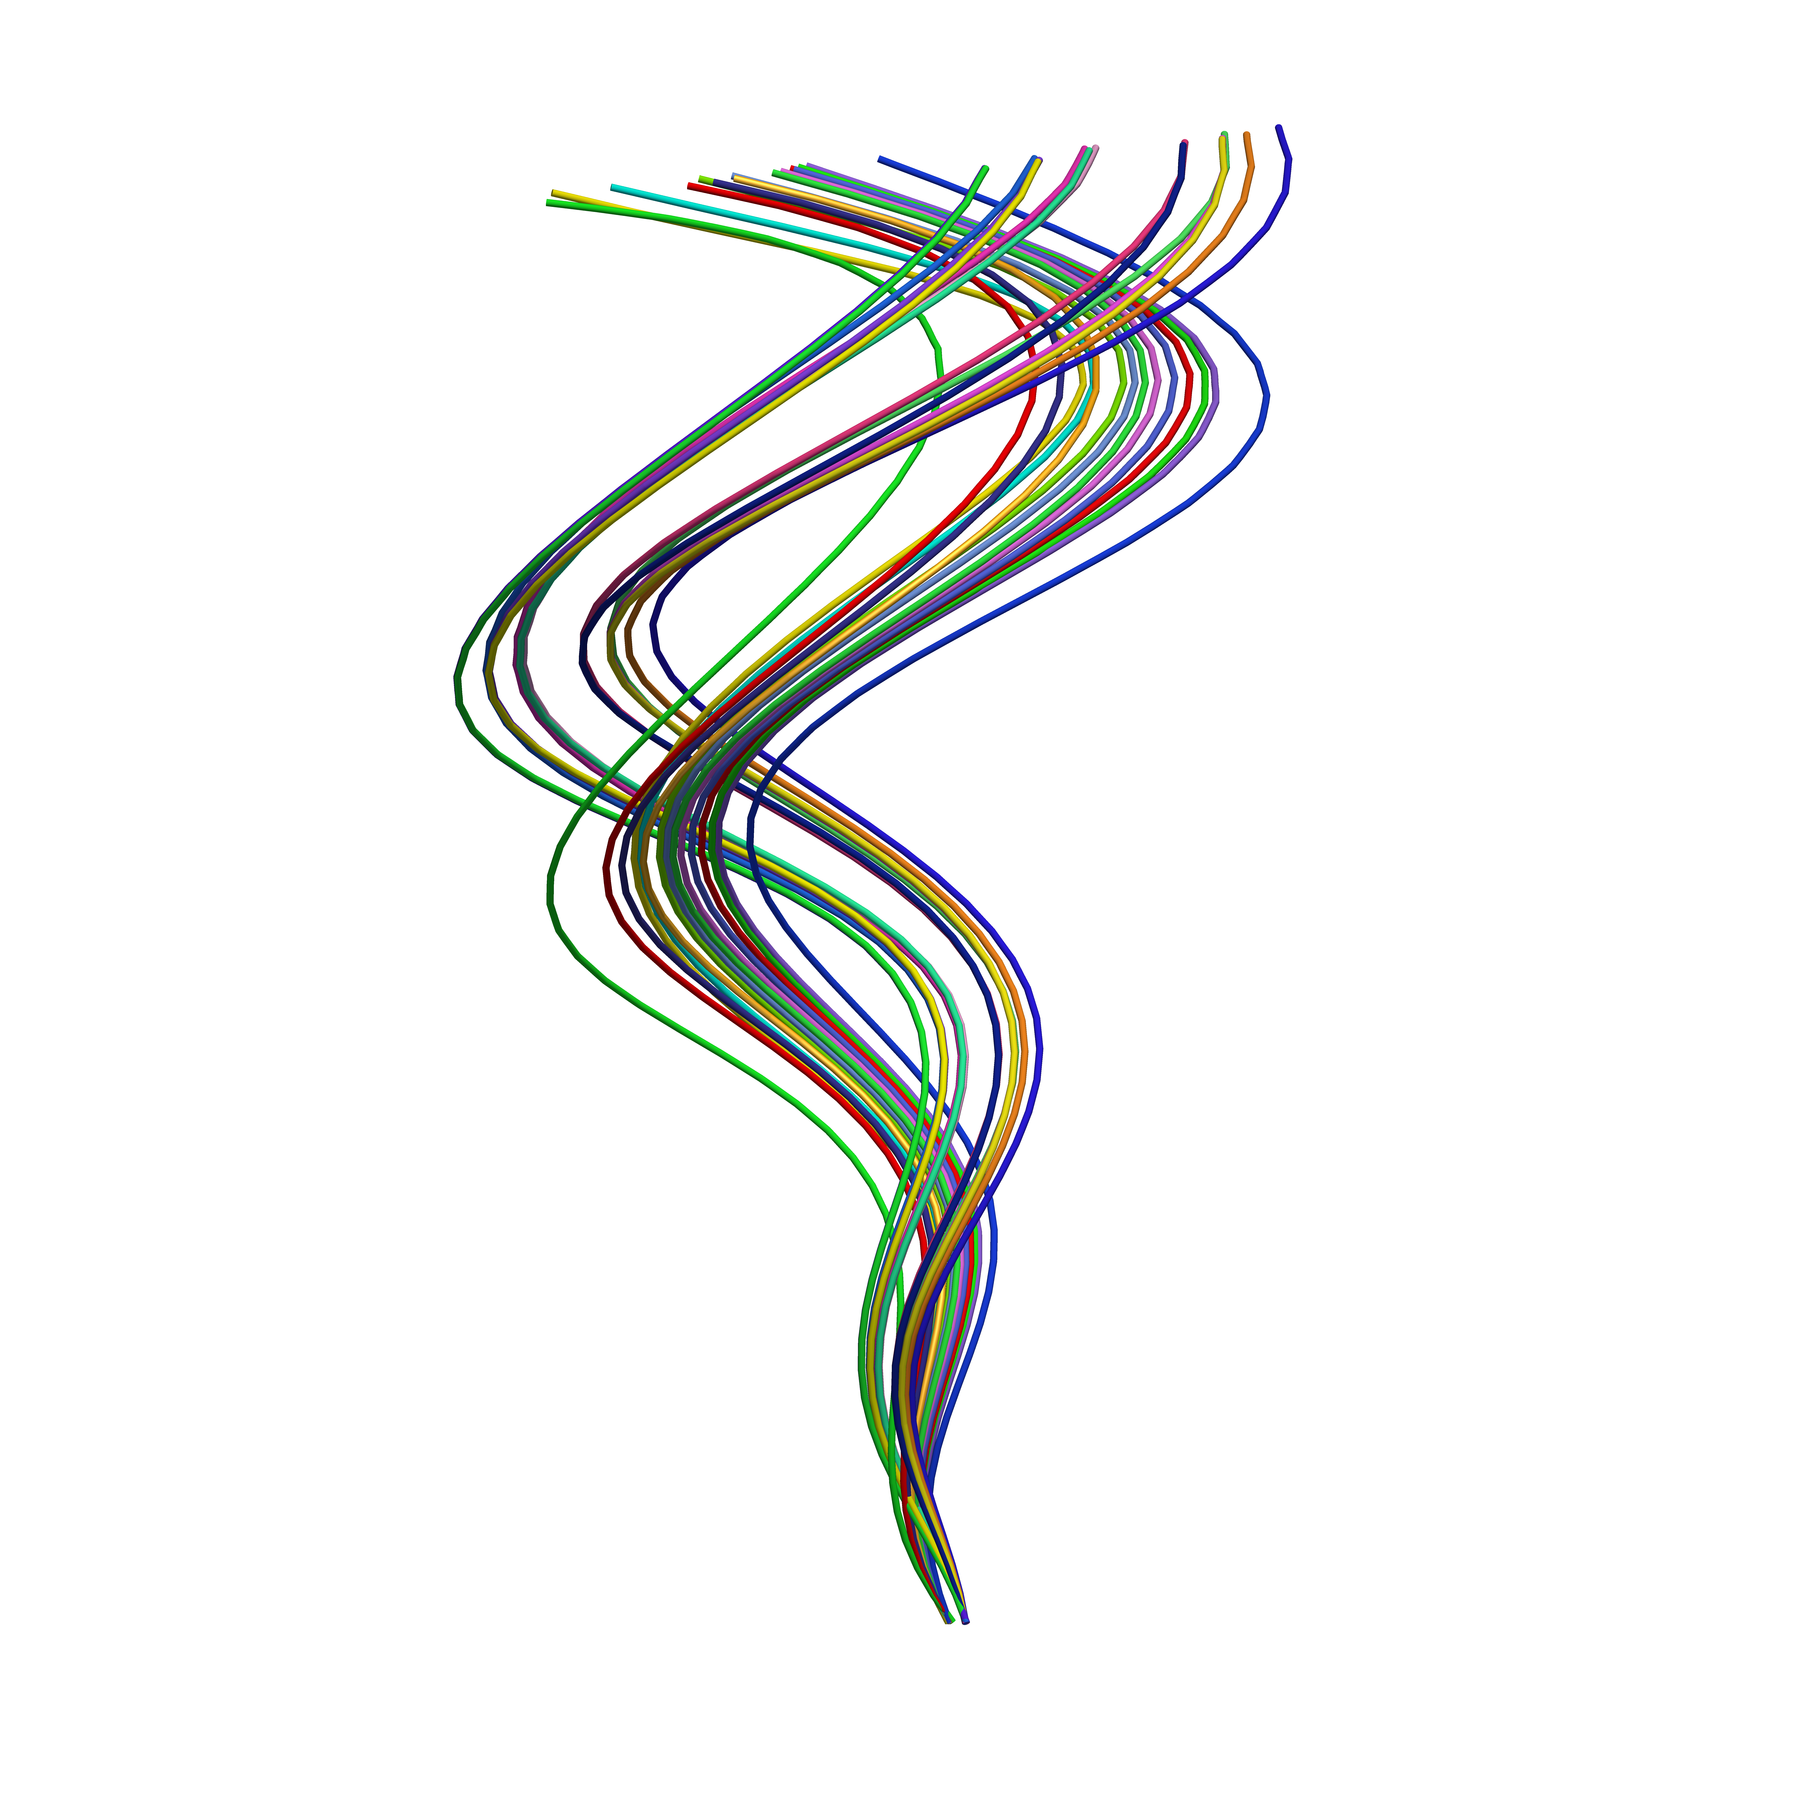
\includegraphics[width=0.75\textwidth]{Images/vcores.png}
    \caption{Spaghetti plot of 30 vortex core lines from a set of flow
    fields. The lines have a similar origin at the bottom of the image,
    but then deviate upwards with increasing differences. The quantity
    of the variance is not easily determined, as overlapping lines are
    not distinguishable.}
    \label{fig:spaghetti}
\end{figure}
The graphical depiction of uncertainty has for a long time been a field
of visualization, which has not been receiving a lot of attention. But,
with todays available computing power, not only the amount of data
increased, but also the ways in which the data can be aquired. With data
more often coming from simuilations or multiple calculations with
varying parameters, the visualization of uncertainty is of rising
importance. Multiple flows through the same system used to be modeled
with spaghetti plots, yielding a line for each member. Figure
\ref{fig:spaghetti} shows a spaghetti plot of the vortex core lines of
members of an uncertain vector domain. A vortex is a region in which the
flow revolves around a line, the core line. The vortices of these fields
all start at a similar position and then twist upwards with varying
radii and acceleration. The problem with this approach is, that the
united parts are hard to distinguish, unallowing for a decision about
the quantity of uncertainty at a location. With increasing member size,
the image becomes cluttered, but high frequency areas are not
necessarily easy to see and the visualization can not be considered
accurate without indications for error, accuracy of confidence.\\
\indent This was until 2012 Mathias Otto und Holger Theisel presented
their approach for extracting probabilities for the existence of a
vortex core line in a cell. They were the first to expand the
multivariate Gaussian sampling to a neighborhood of a vector field,
giving them normally distributed derivatives. This allowed them to
process their sampled cells using the Parallel Vectors operator, to find
the points at which the velocity vector is parallel to its derived
acceleration vector. If now the Jacobian matrix at the found point has a
pair of complex conjugate eigenvalues, the point lies on a vortex.
Complex eigenvalues denote a rotational transformation. The relative
number of positive samples are then the probability for a vortex core
line in that cell. Figure~\ref{fig:UVC} shows the result of the
uncertain vortex calculation for the whole set of vector fields from
Figure~\ref{fig:spaghetti}. The set is very uncertain. As the vortices
all have a similar base and start to deviate upwards, there are red
region with high probability at the bottom. From there on up, the lines
spread and therefore there are wider regions with low probability. This
directly highlights common regions of the individual members and eases
the understanding of the uncertainty in the fields.\\
\indent As the derivative of a scalar field is a vector field, an idea
that comes to mind is to apply their method to the extraction of
features from uncertain scalar fields. For the extraction of a ridge
line from an 3-dimensional scalar field, the approach is basically the
same. We only require an extra step, calculating the gradient of the
sampled scalar field, to get an uncertain vector field in which we can
search for similar criteria. The Parallel Vectors operator is easily
adjusted to give the points where the gradient is parallel to its major
eigenvector and the eigenvalues of the Hessian, the counterpart to the
Jacobian, don't need to be complex, but negative. The extraction of a
ridge surfaces on the other hand is a bit different as we are searching
for orthogonality of the gradient and the minor eigenvector. An adjusted
variant of the Marching Cubes algorithm would give us an approximation
of the uncertain ridge surface, but this method has some problems,
especially at volatile locations of the fields, where the ridge of the
individual members is already weak. The next chapter will give detailed
information on the problems coming with Uncertain Marching Cubes and how
we tried to overcome them.

\begin{figure}[t]
    \centering
    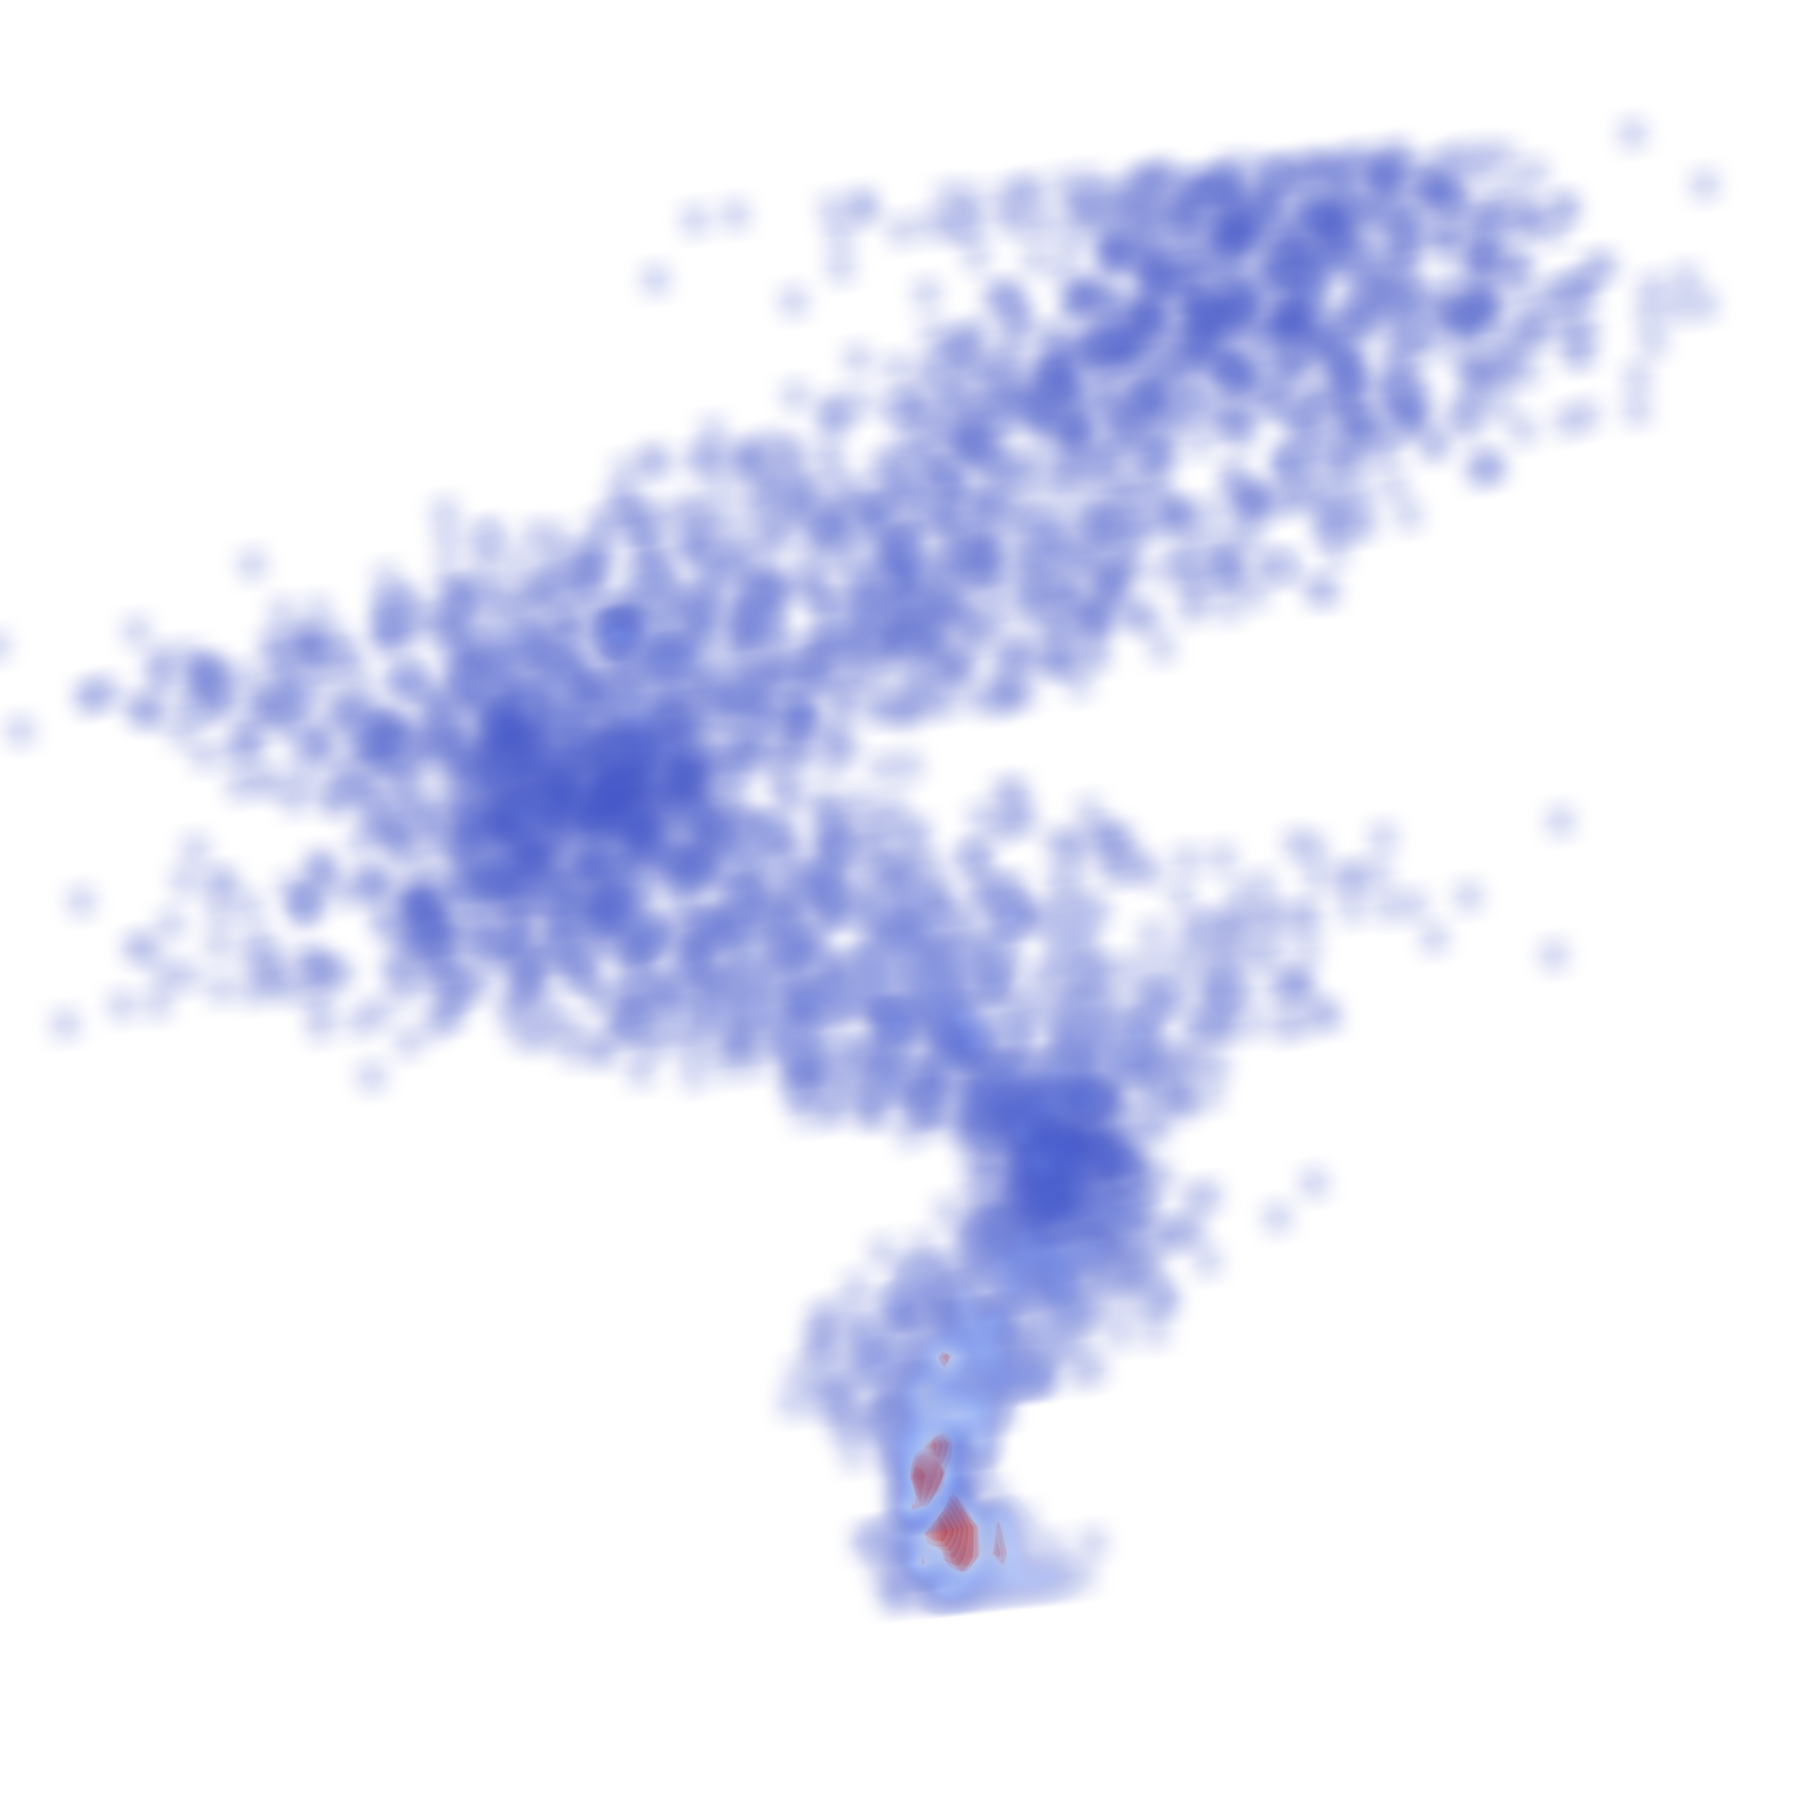
\includegraphics[width=0.75\textwidth]{Images/unccores.png}
    \caption{Uncertain vortex core lines for the full set of correlated
    flow fields. Region with probability reaching $100\%$ at the bottom,
    where the core lines originate. The individual lines originate from
    minor changes of the general direction and radius. As the line expands
    upwards, these changes become more and more visible, leading to an
    increasind spread of the uncertain visualization.}
    \label{fig:UVC}
\end{figure}
  %%%%%%%%%%%%%%%%%%%%%%%%%%%%%%%%%%%%%%%%%%%%%%%%%%%%%%%%%%%%%%%%%%%%%%%%
\chapter{Method}
%%%%%%%%%%%%%%%%%%%%%%%%%%%%%%%%%%%%%%%%%%%%%%%%%%%%%%%%%%%%%%%%%%%%%%%%

Method and stuff.

  %%%%%%%%%%%%%%%%%%%%%%%%%%%%%%%%%%%%%%%%%%%%%%%%%%%%%%%%%%%%%%%%%%%%%%%%
\chapter{Evaluation}\label{chap:Eval}
%%%%%%%%%%%%%%%%%%%%%%%%%%%%%%%%%%%%%%%%%%%%%%%%%%%%%%%%%%%%%%%%%%%%%%%%

This chapter will evaluate the results obtained with our new criterion,
compare them with the conventional method, as well as show its vantages
and disadvantages. But at first, we will talk about the differences of
the matrix decompositions used to generate the samples from the
multivariate distributions.

%%%%%%%%%%%%%%%%%%%%%%%%%%%%%%%%%%%%%%%%%%%%%%%%%%%%%%%%%%%%%%%%%%%%%%%%
\section{Comparison of Matrix Decompositions}\label{chap:evalMD}
%%%%%%%%%%%%%%%%%%%%%%%%%%%%%%%%%%%%%%%%%%%%%%%%%%%%%%%%%%%%%%%%%%%%%%%%

Multivariate Gaussian sampling is a common way to model distributions
by drawing variants from the set. This method makes use of the
factorization of the covariance matrix $\Sigma$ from the distribution into
the product of two matrices, such that $\Sigma = AA^\top$. Literature
like ``Random Number Generation and Monte Carlo Methods''~\cite{Monte}
state, that any decomposition that achieves such a factorization is
suitable for the genration of random samples and delivers equally
good results. Therefore one could prefer the Cholesky decomposition
because of its faster computation time $\mathcal{O}(N^3/3)$ over
the Eigendecomposition with $\mathcal{O}(N^3)$. To compare the two
decompositions, we take the function from Figure~\ref{fig:sfield} and
equally shift it along the $x$-dimension to create a set of twenty
members with a high uncertainty along $x$, but no uncertainty along
the other dimensions, ridgewise. Figure~\ref{fig:decomps} shows the
result of the uncertain ridge calculation for both decompositions using
the new criterion. The surfaces exhibit heavy differences. While the
Eigendecomposition deliveres a smooth estimation with a constant high
probability for the ridges that every field contains and a blue cloud
with low probability where the ridge is uncertain, Cholesky has a
distorted ridge perpendicular to $y$ as well as three to four distinct
ridge structures across $x$ with a low probability. The result of the
Cholesky decomposition is considerably worse.

\begin{figure}
    \begin{subfigure}[b]{0.49\textwidth}
        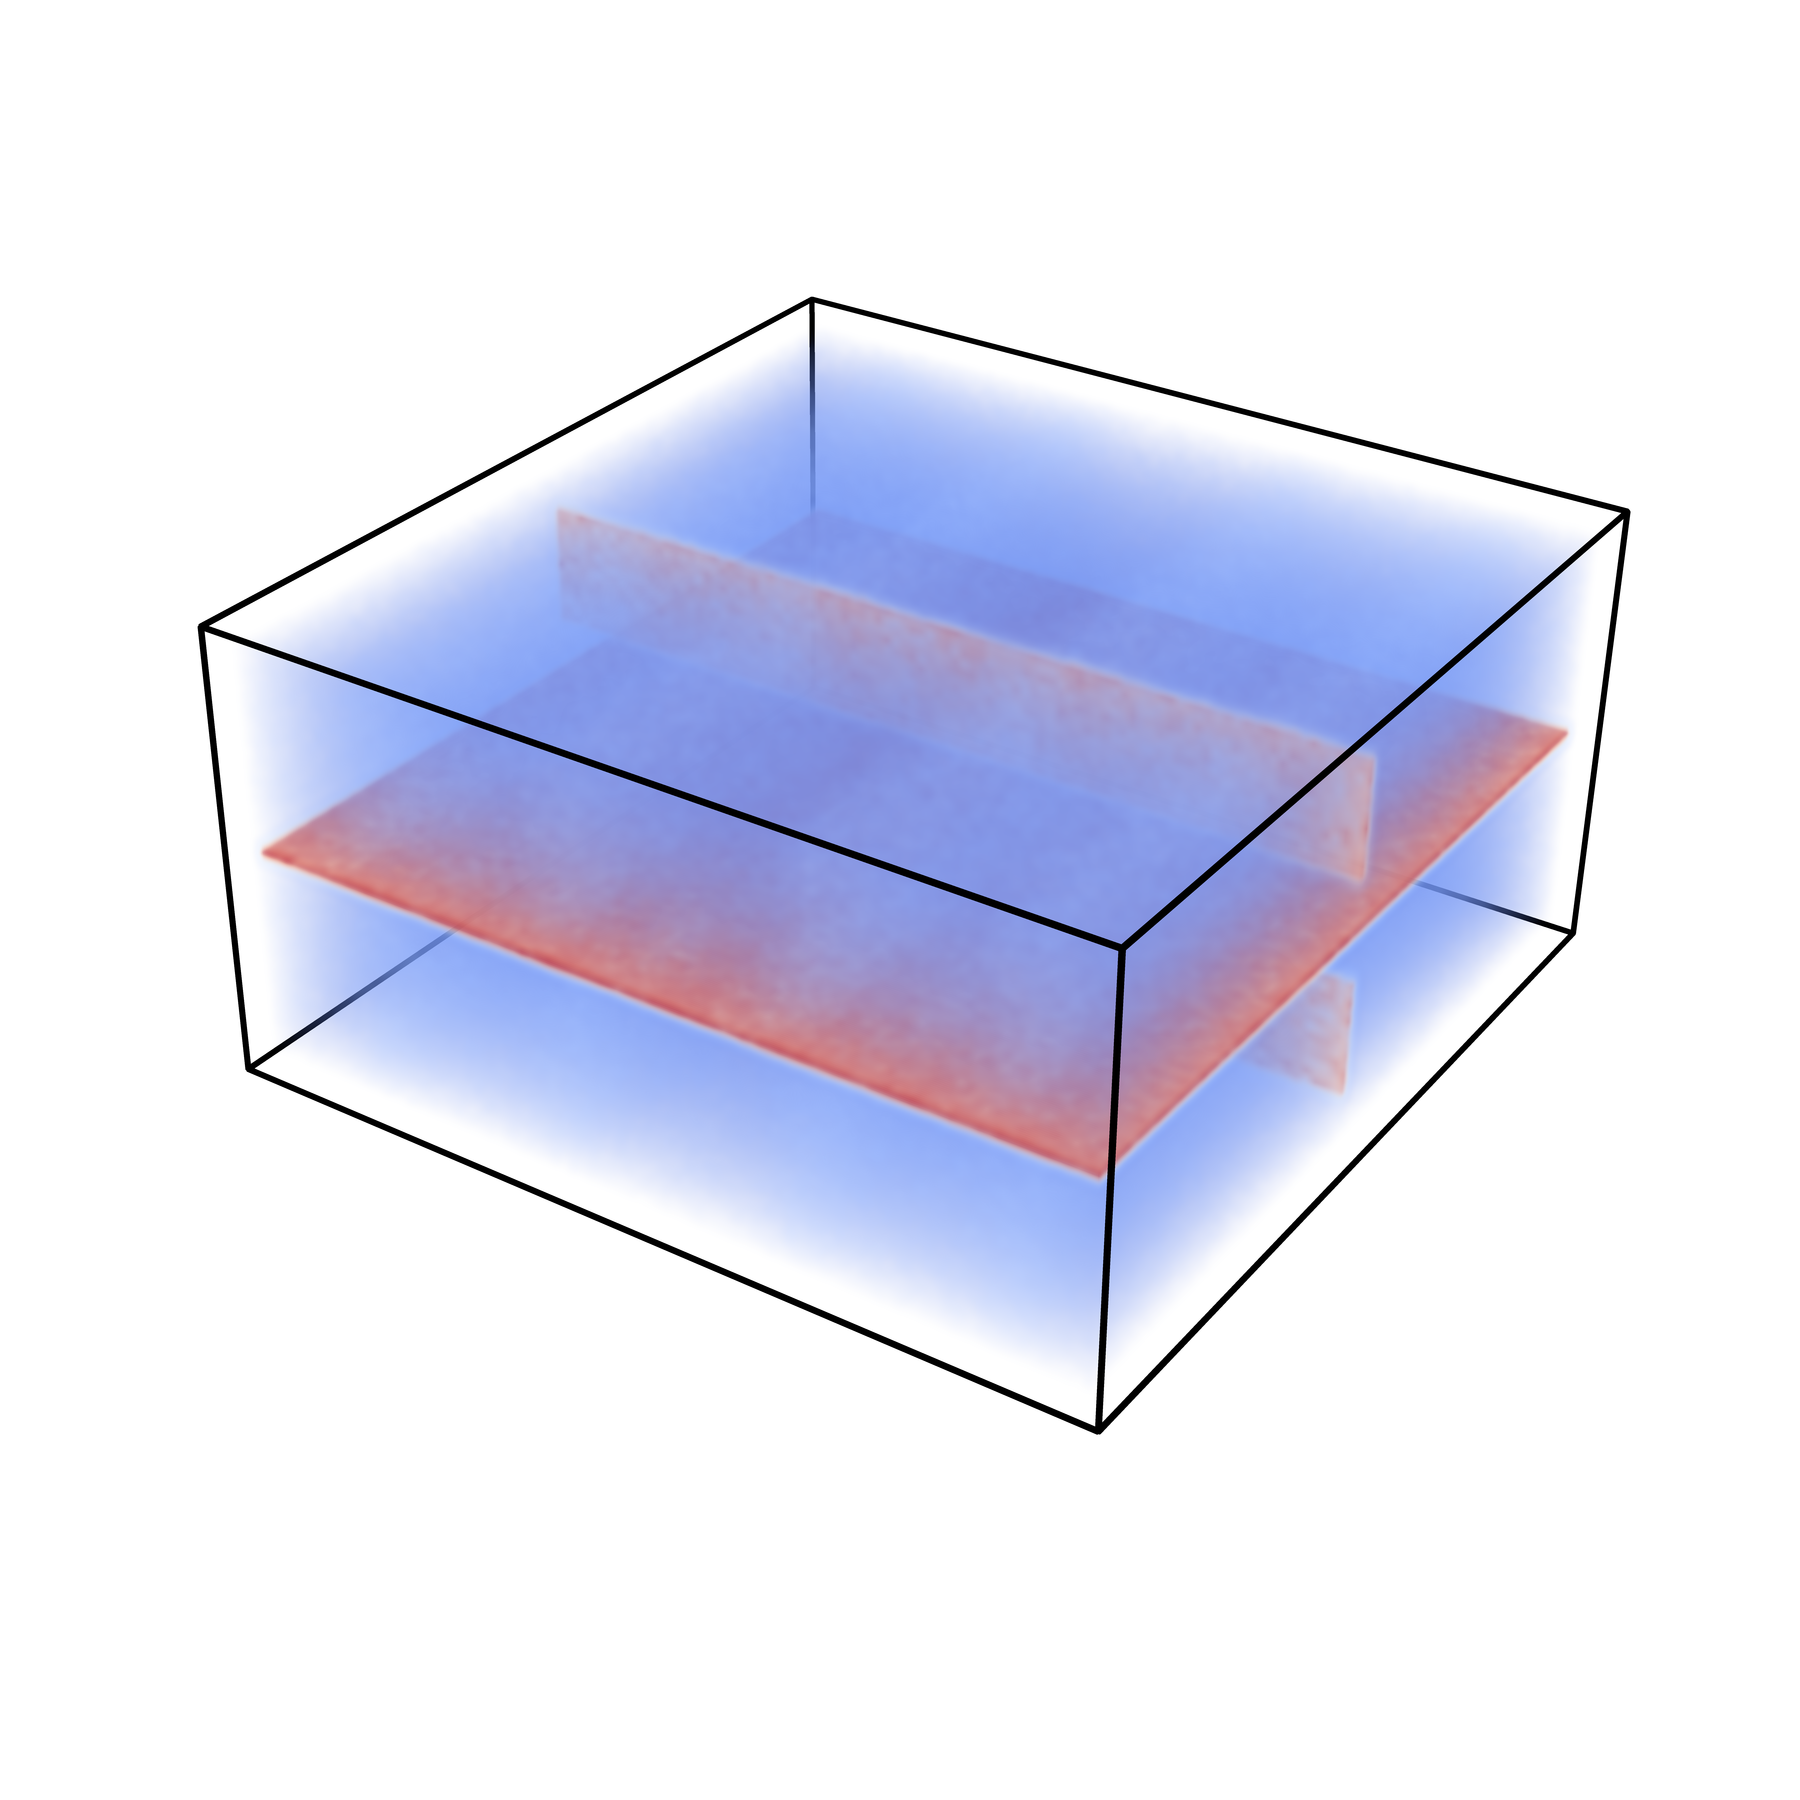
\includegraphics[width=\textwidth]{Images/shiftXeigen.png}
        \caption{Eigendecomposition}
        \label{fig:shiftXeigen}
    \end{subfigure}
    \begin{subfigure}[b]{0.49\textwidth}
        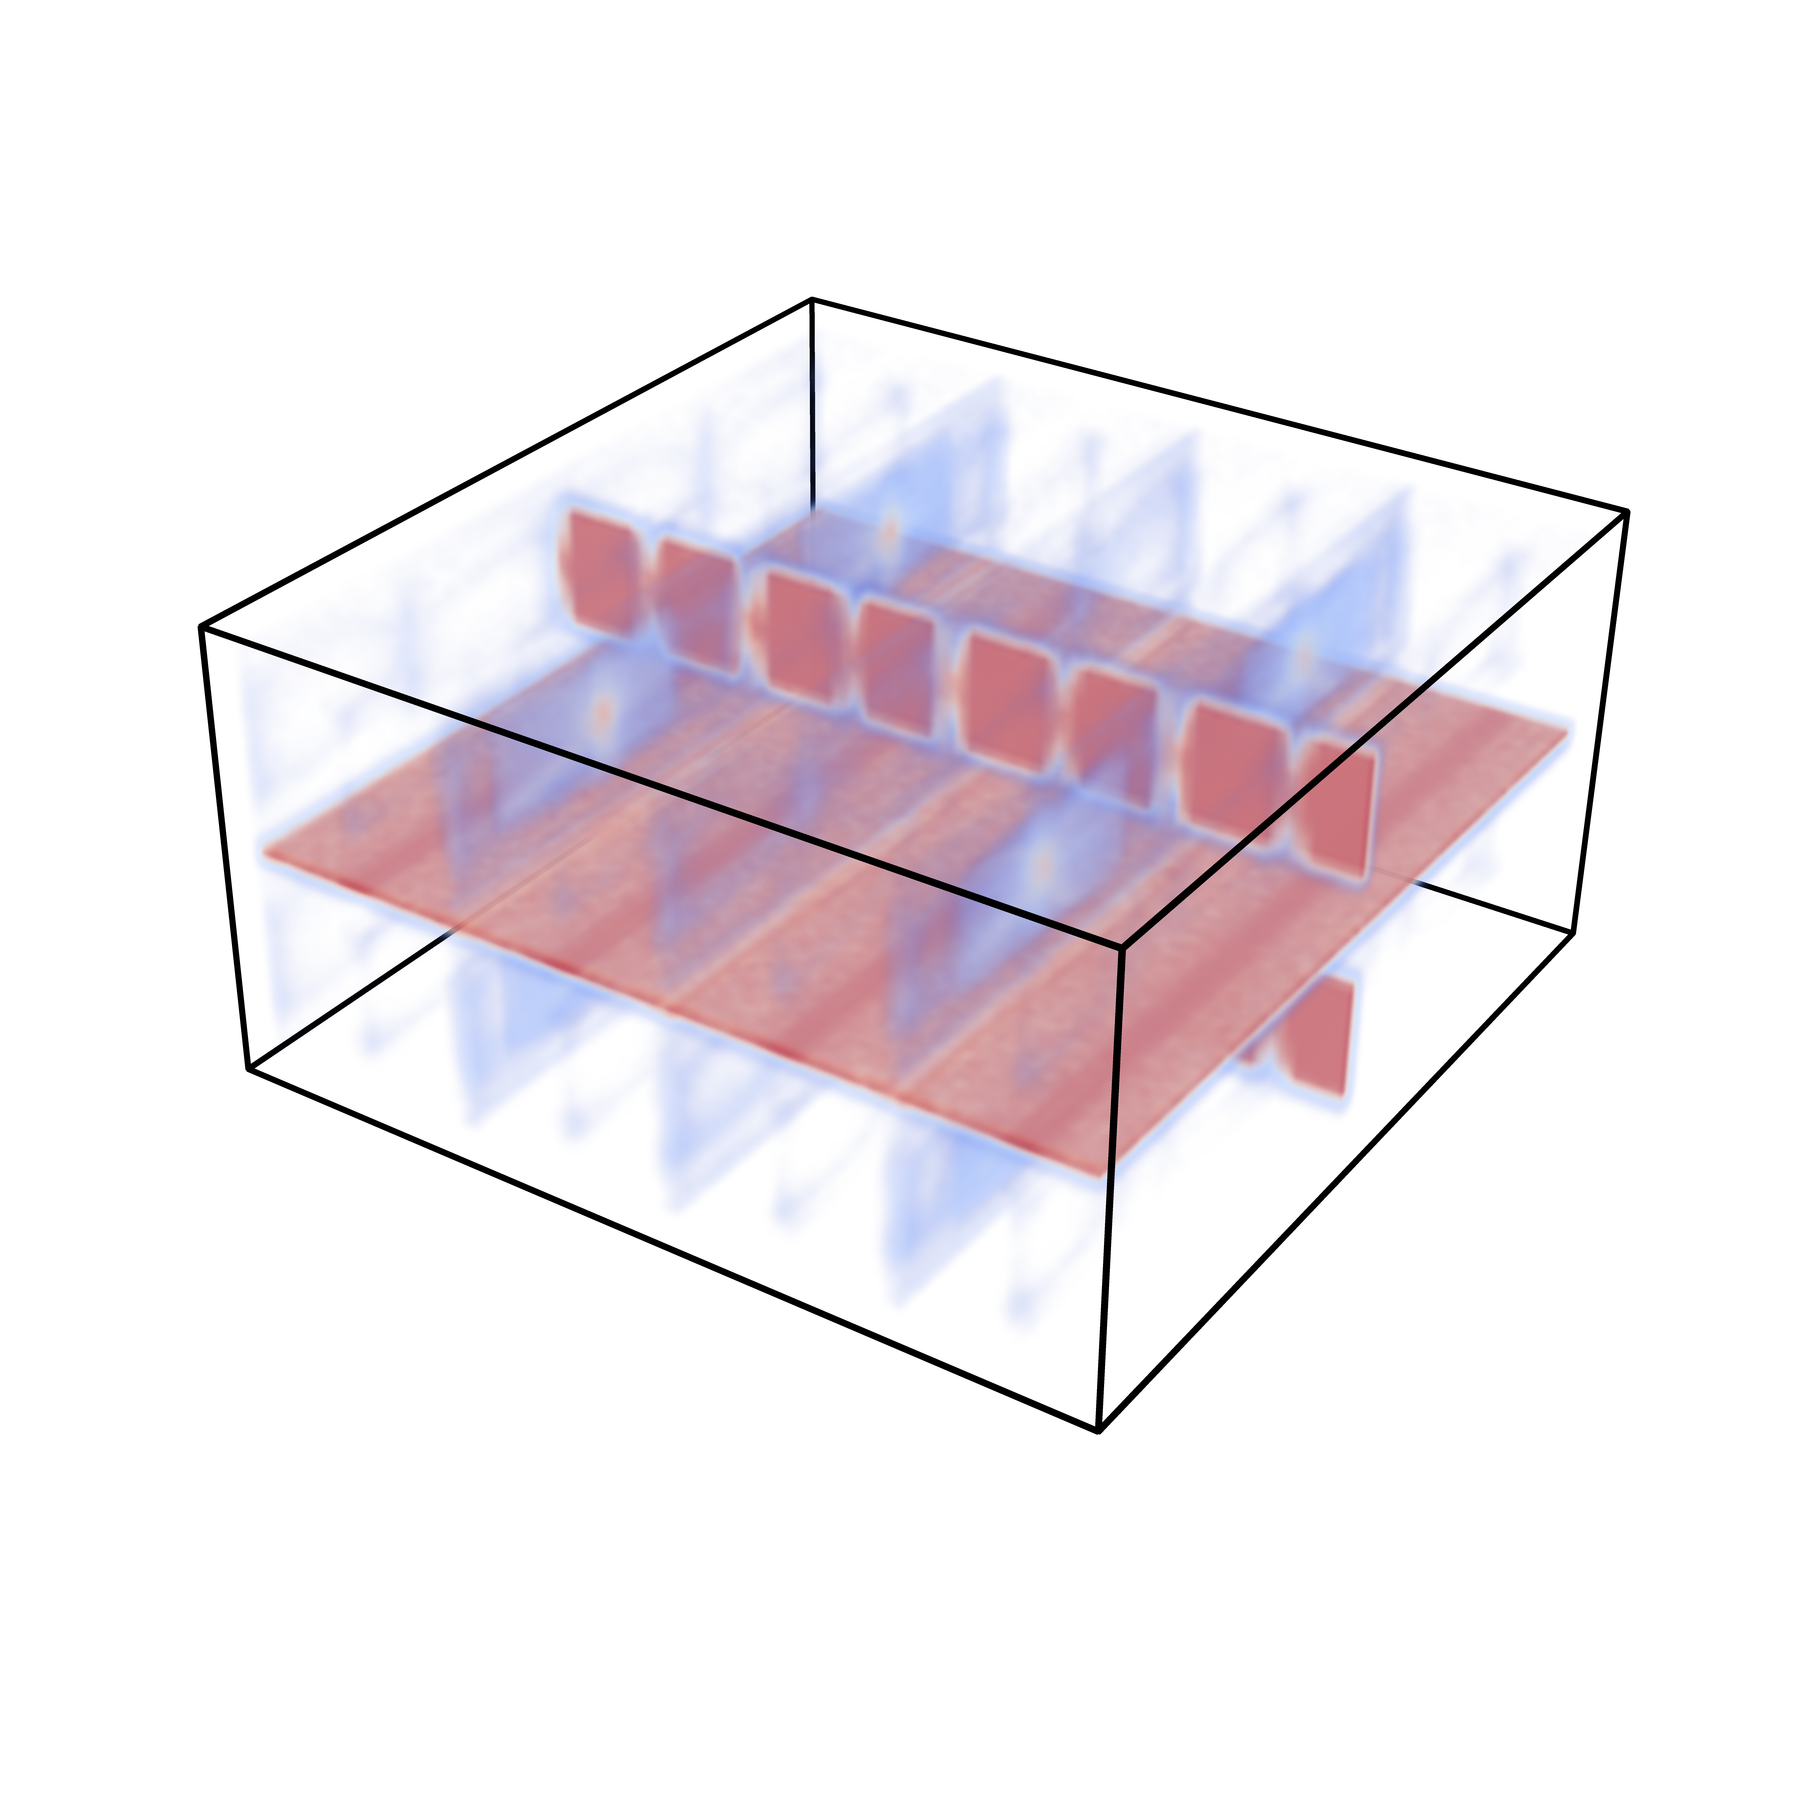
\includegraphics[width=\textwidth]{Images/shiftXcholesky.png}
        \caption{Cholesky}
        \label{fig:shiftXcholesky}
    \end{subfigure}
    \caption{Comparison of the two matrix decompositions for a set
    of fields shifted equally along the $x$ dimension. The 
    Eigendecomposition gives a smooth estimate of the ridge surface,
    according to the distribution of the ridges in the members.
    Cholesky exhibits lower probabilities at points where the
    ridge is very certain.}
    \label{fig:decomps}
\end{figure}

\noindent To understand what happened here, we will again take a look at
samples drawn from the distribution of Figure~\ref{fig:sampComp}.
Figure~\ref{fig:MDsampComp} shows the gradients of two samples from
either decomposition with their respective unscaled eigenvectors at the
base. Even though the Eigendecomposition in Figure~\ref{fig:sampleEig}
breaks the parallelity of the original field, the gradients still point
in the same general direction and the eigenvectors are consistently
oriented. The gradients of Cholesky on the other hand have no
directional correlation at all. The direction of the vectors is
arbitrary along the distribution and therefore their eigenvectors
have inconsistent orienting as well. The Eigendecomposition seems
to keep the correlation of elements of individual members, whereas
Cholesky mingles the members in one sample. For the calculation of
a ridge feature which depends on precision, this is an issue. The
differences are the consequence of the immanent nature of the
decompositions. The Eigendecomposition of the covariance matrix
equals to the Principal Component Analysis and therefore the scaled
eigenvectors equal to the uncertainty of $\Sigma$ along
the direction of the eigenvector. If we now multiply a standard normal
distributed vector $N$ with $A = E\Lambda$, every $i$-th component of
$N$ is multiplied with a component of the $i$-th column of $A$, and thus
the $i$-th eigenvector. This leads to a constant scaling of elements
along the direction of the eigenvectors. Cholesky produces a lower
triangular matrix for $A=LD^{\frac{1}{2}}$, thus the columns have
increasing influence on the distribution of the sample with increasing
$i$, but the first element of the sample vector is only determined by
the scaling of $a_{11}$ with the random number at $N_1$. An interesting
implementation detail is, that the algorithm calculating the eigenvalues
for our large covariance matrices uses the power iteration method, that
estimates the largest absolute eigenvalue $\lambda$ in $\mathcal{O}
(N^2)$. Then the matrix is reduced by $A-\lambda I$ and power iteration
is applied again. This process can be repeated until all eigenvalues are
found. Analytic results are too computationally intensive for matrices
of size $80 \times 80$ or $24 \times 24$. Due to this algorithm, the
first column of our eigenvectormatrix always corresponds to the largest
eigenvalue, and therefore the axis with the greatest variance of the
set. Comparing this to the Cholesky decomposition, we could say that the
samples from Cholesky are mainly influenced by one axis of variance of
the data set, and decreasingly influenced by the latter variances,
resulting in more random samples. Ond\v{r}ej Straka \etal{\cite{MD}}
studied the different matrix decompositions in the context of Unscented
Kalman Filters, but their results are applicable for our case as well.
They drew three conclusions after their analysis of the decompositions:
If the variable we want to sample contains no correlated elements, the
samples for both decompositions are equally good and therefore the
Cholesky decomposition might be prefered because of its faster
computation time. If the variable contains correlated elements, the
choice may significantly affect the quality of the sample and if the
elements exhibit strong correlation, numerical stability becomes an
issue as well, especially for Cholesky. Considering, that we usually
apply the uncertain ridge extraction to data sets obtained from
simulations, we will have strong correlation of the members of the data
set for the most parts of the field. We will talk about the numerical
stability in Chapter~\ref{chap:Discu}. The difference of the
decompositions is particularly visible when comparing the results
obtained from the ridge extraction using Marching Cubes
(Figure~\ref{fig:MCcomp}). Cholesky produces the same structure as in
Figure~\ref{fig:shiftXcholesky}, but with more certainty. This is a
misleading representation of the underlying uncertainty. The results
obtained from the Eigendecomposition (Figure~\ref{fig:MCeigen}) on the
other hand can almost be considered better than the ones with our new
criterion, as the high probabilities are notably thinner distributed,
just like the certain ridge would be. We will compare the two approaches
in the next section. Concluding from all of this, the Eigendecomposition
delivers better results in most cases. Only if we have strong uncertainty
in the data, the Cholesky decomposition may give us better results.
We took the set from Figure~\ref{fig:MCridges} and extended it with
members having greater variance along either axis. The results of the
two decompositions can be seen in Figure~\ref{fig:HUCcomp}. Here
Cholesky gives us higher probabilities for nodes close to the mean of
the ridges. Due to the high variance of the data set, the members seem
to lose their correlation. The downside is, that this case is not the
usual thing for real world data, where we try to extract ridge structures
from similar scalar fields. 

\begin{figure}
    \begin{subfigure}[b]{0.49\textwidth}
        \includegraphics[width=\textwidth]{Images/sampleEig.png}
        \caption{Eigendecomposition}
        \label{fig:sampleEig}
    \end{subfigure}
    \centering
    \begin{subfigure}[b]{0.49\textwidth}
        \includegraphics[width=\textwidth]{Images/sampleChol.png}
        \caption{Cholesky}
        \label{fig:sampleChol}
    \end{subfigure}
    \caption{Gradients of samples from the distribution of the rotated
    field for $f(x,y)=x^2$. The samples from the Eigendecomposition
    keep the structure of the original fields, whereas the Cholesky
    decomposition mixes the distributions in one sample.}
    \label{fig:MDsampComp}
\end{figure}

\begin{figure}
    \begin{subfigure}[b]{0.49\textwidth}
        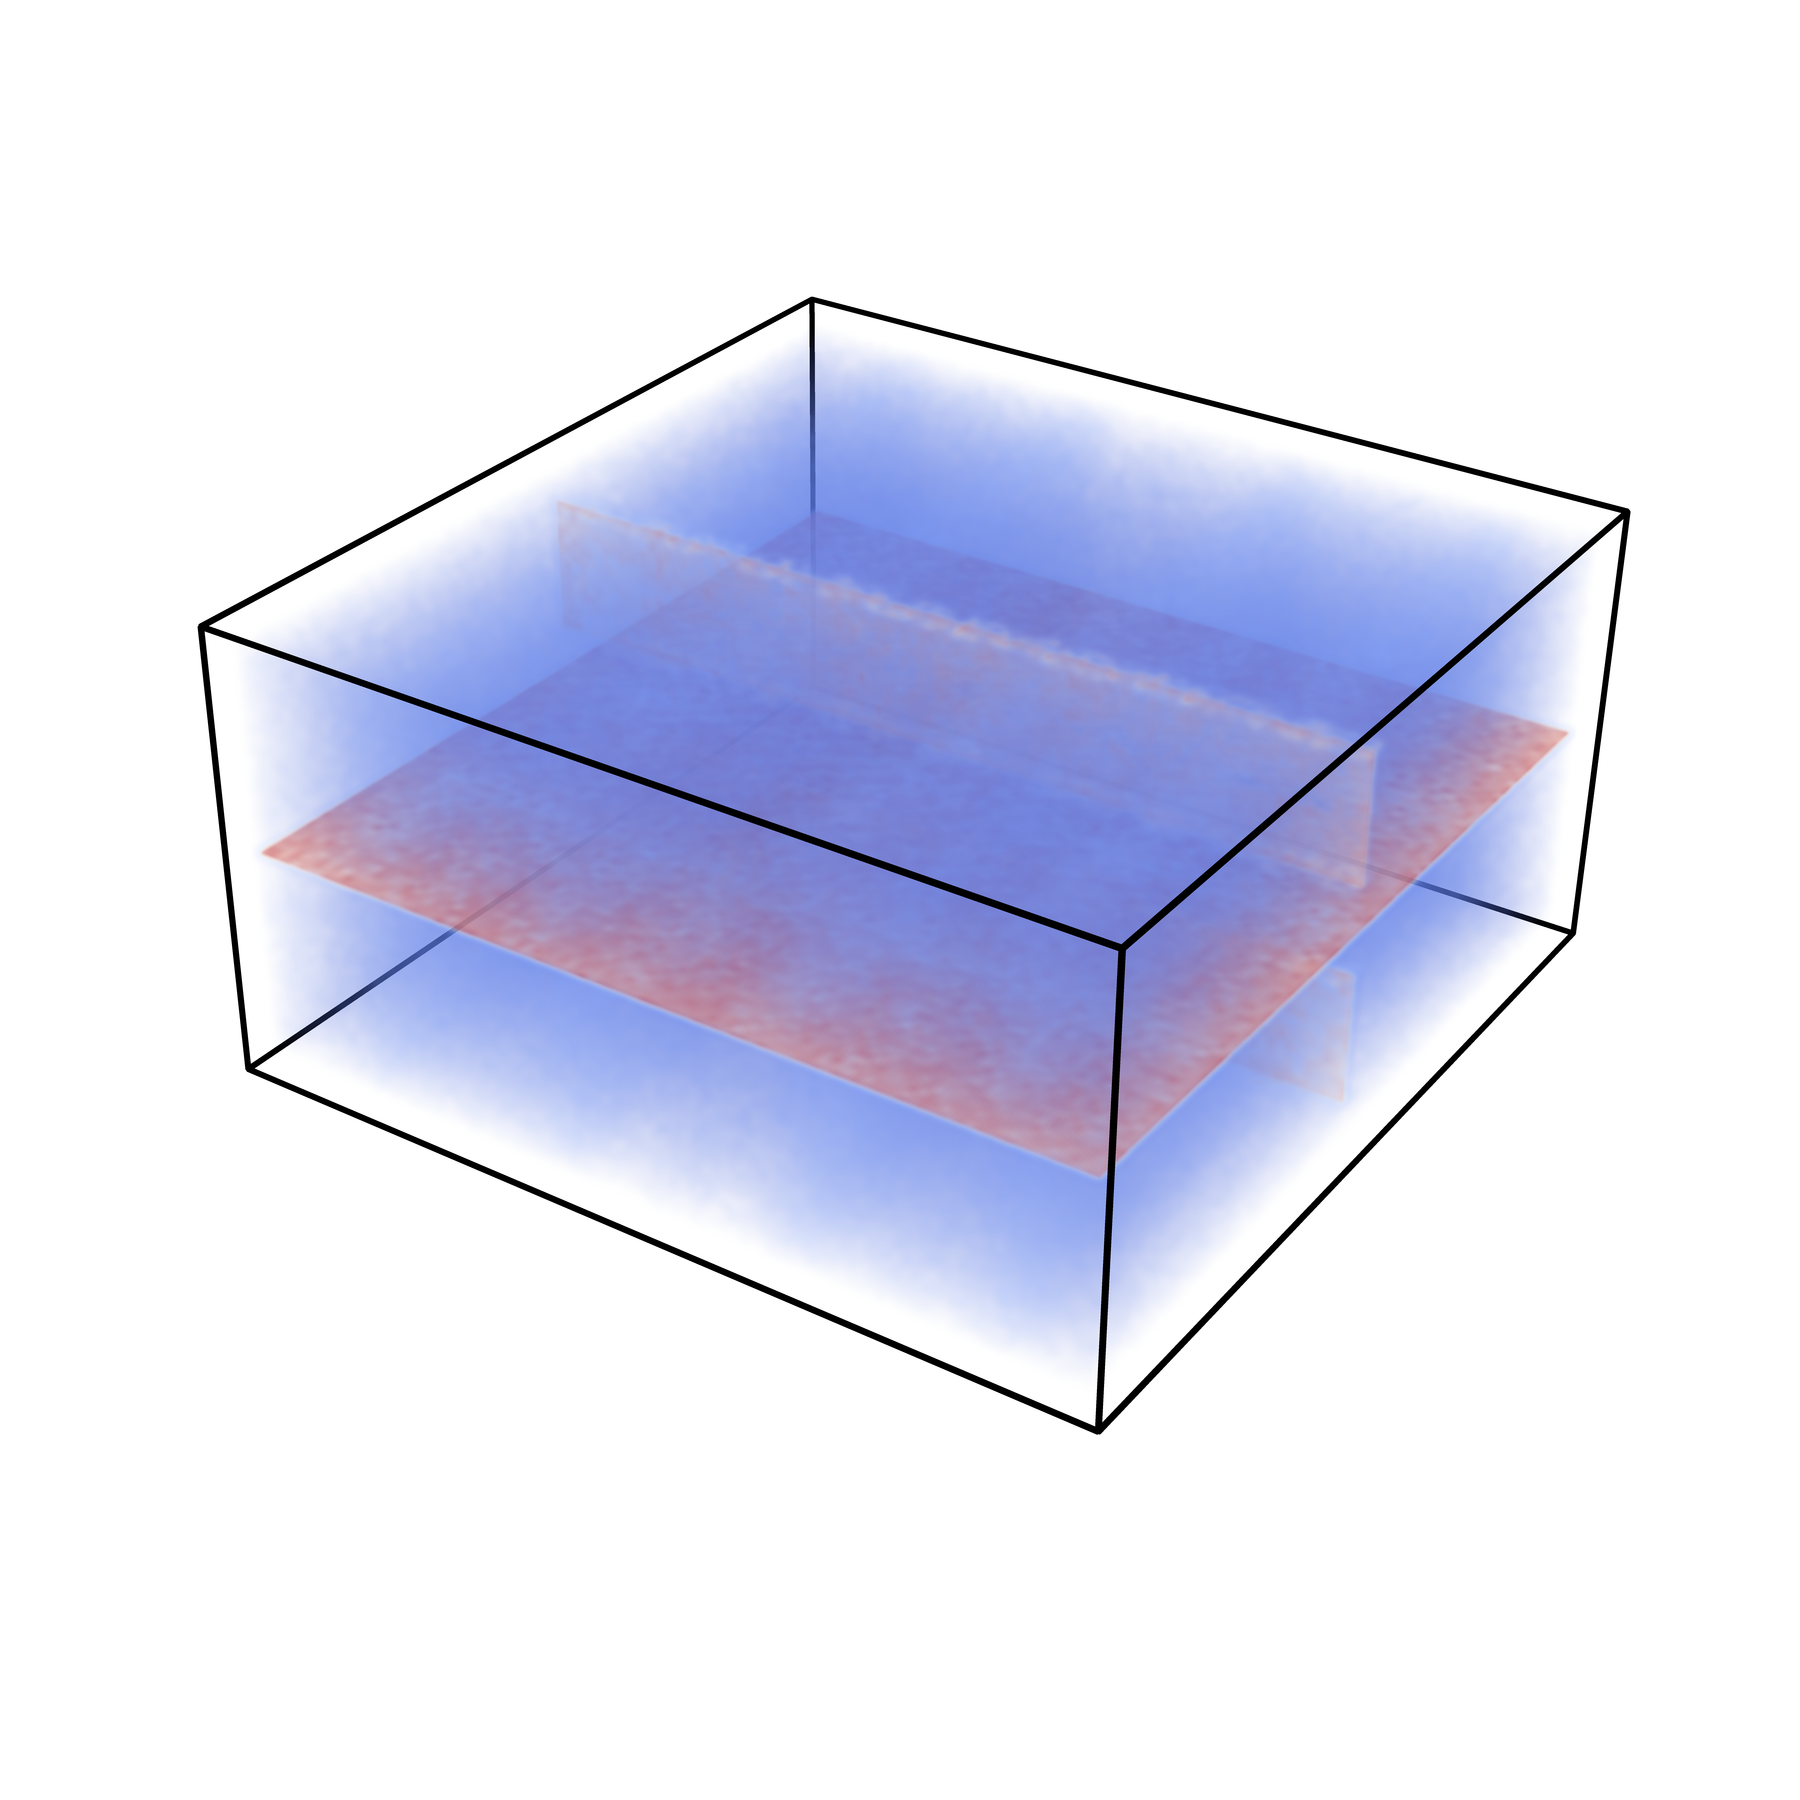
\includegraphics[width=\textwidth]{Images/shiftXold.png}
        \caption{Eigendecomposition}
        \label{fig:MCeigen}
    \end{subfigure}
    \begin{subfigure}[b]{0.49\textwidth}
        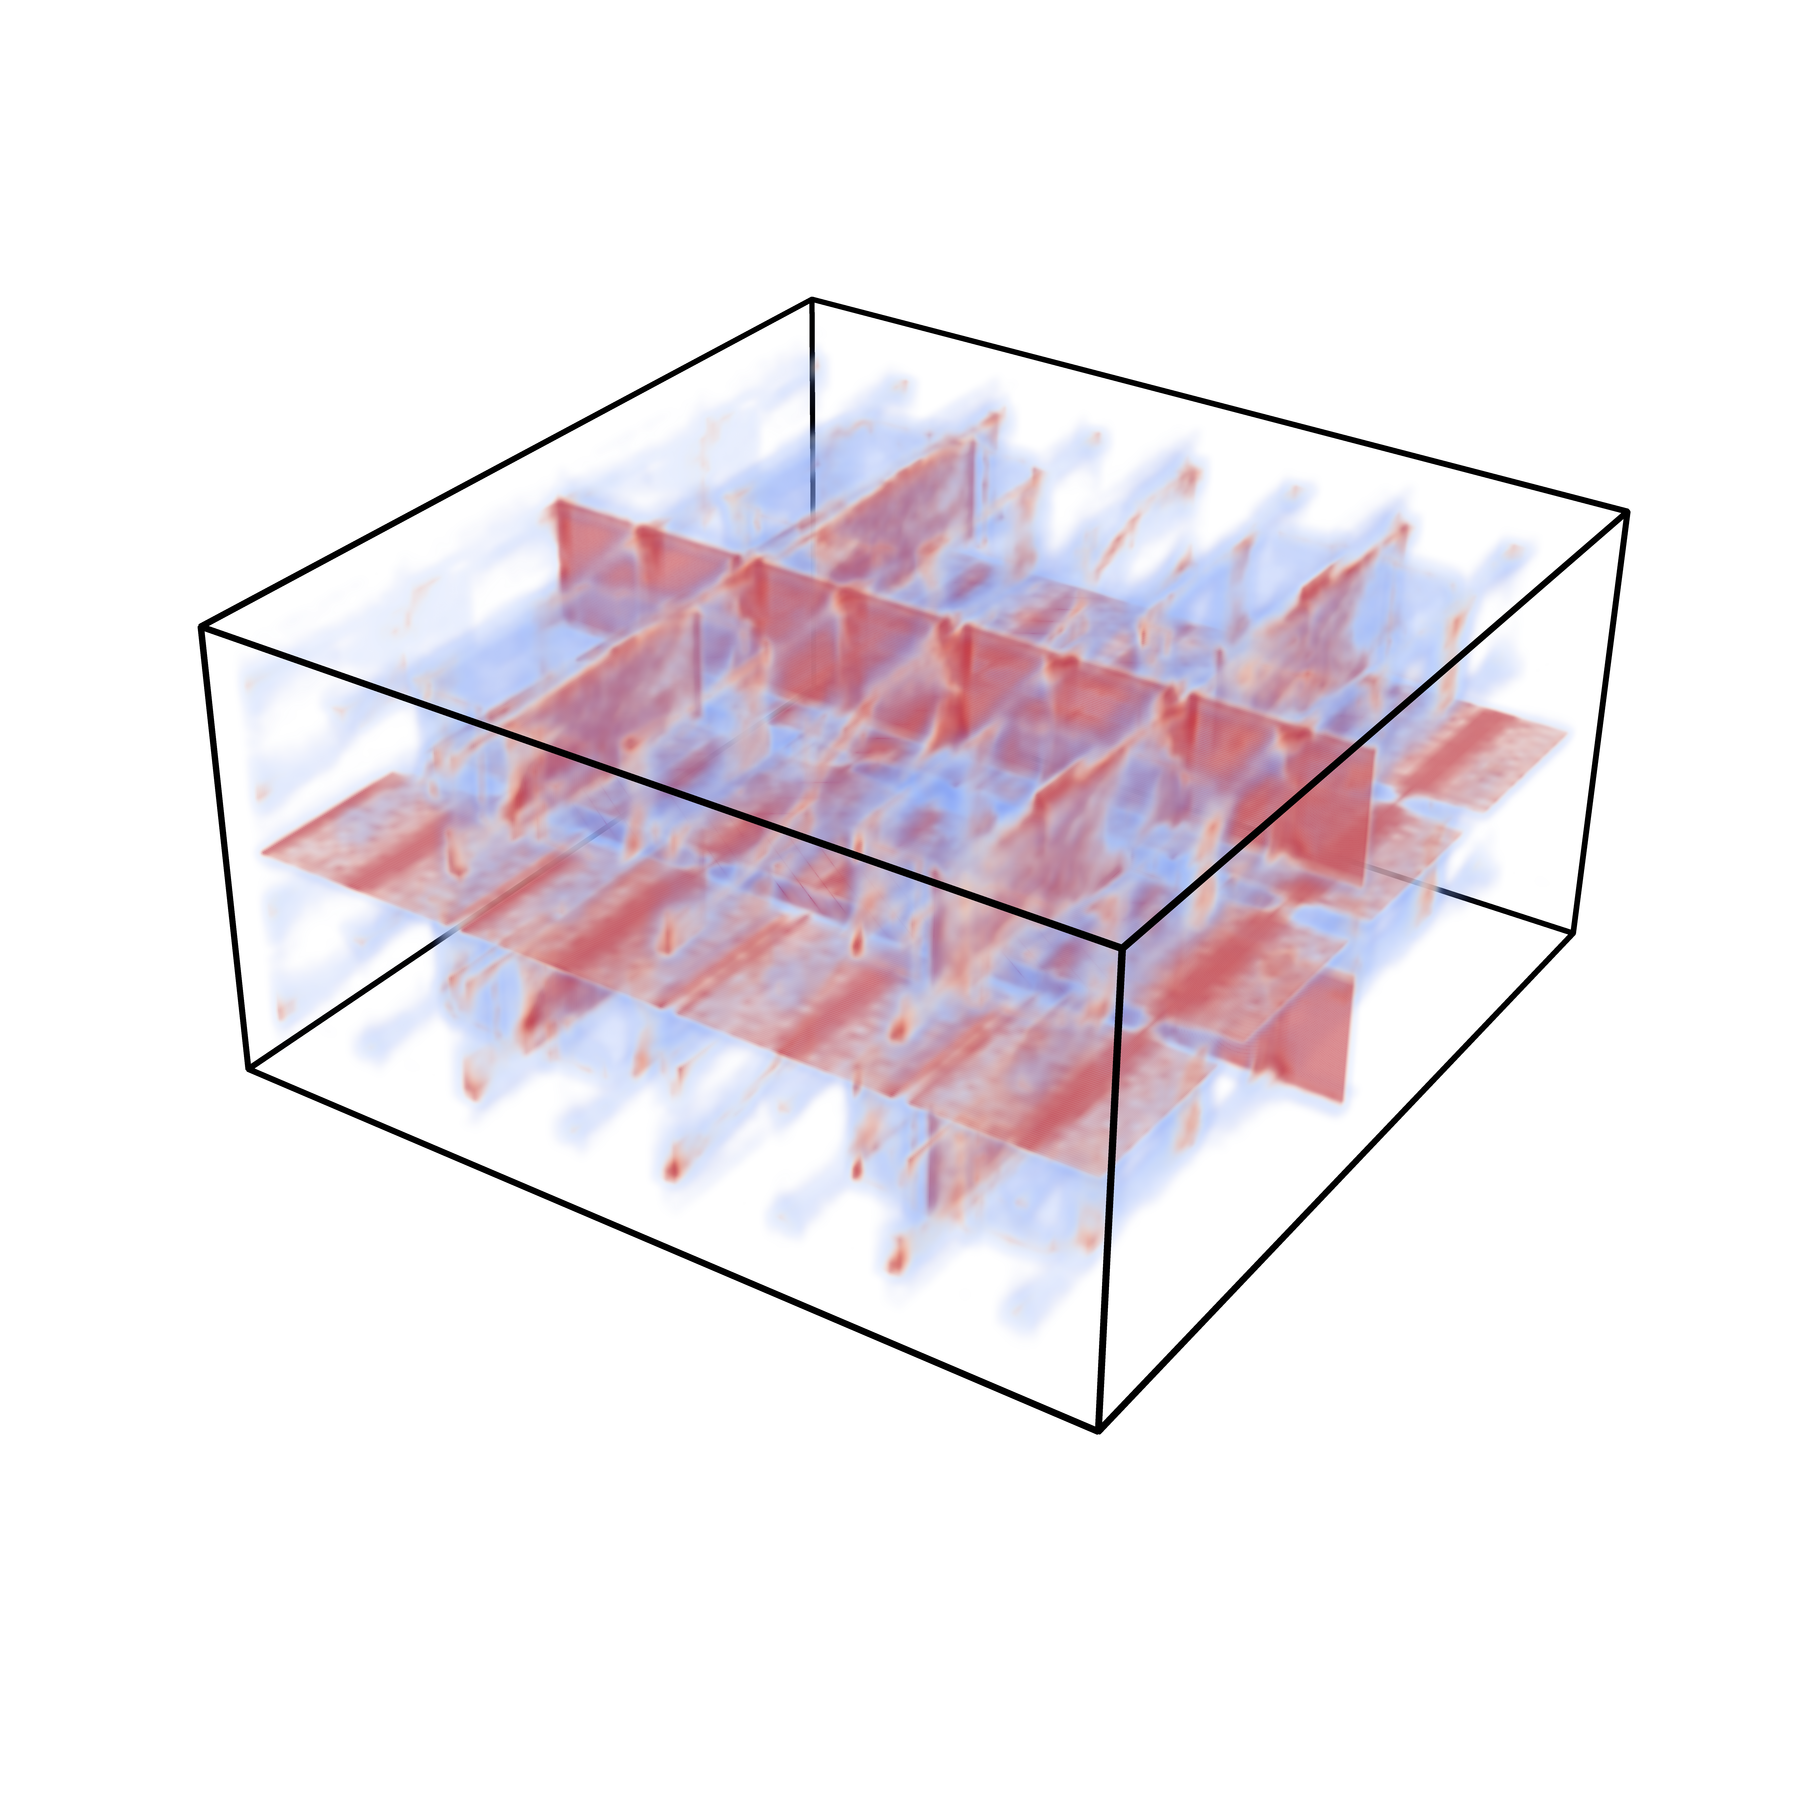
\includegraphics[width=\textwidth]{Images/shiftXoldchol.png}
        \caption{Cholesky}
        \label{fig:MCchol}
    \end{subfigure}
    \caption{Comparison of matrix decompositions for the uncertain
    ridge extraction using the Marching Cubes algorithm.}
    \label{fig:MCcomp}
\end{figure}

\begin{figure}
    \begin{subfigure}[b]{0.49\textwidth}
        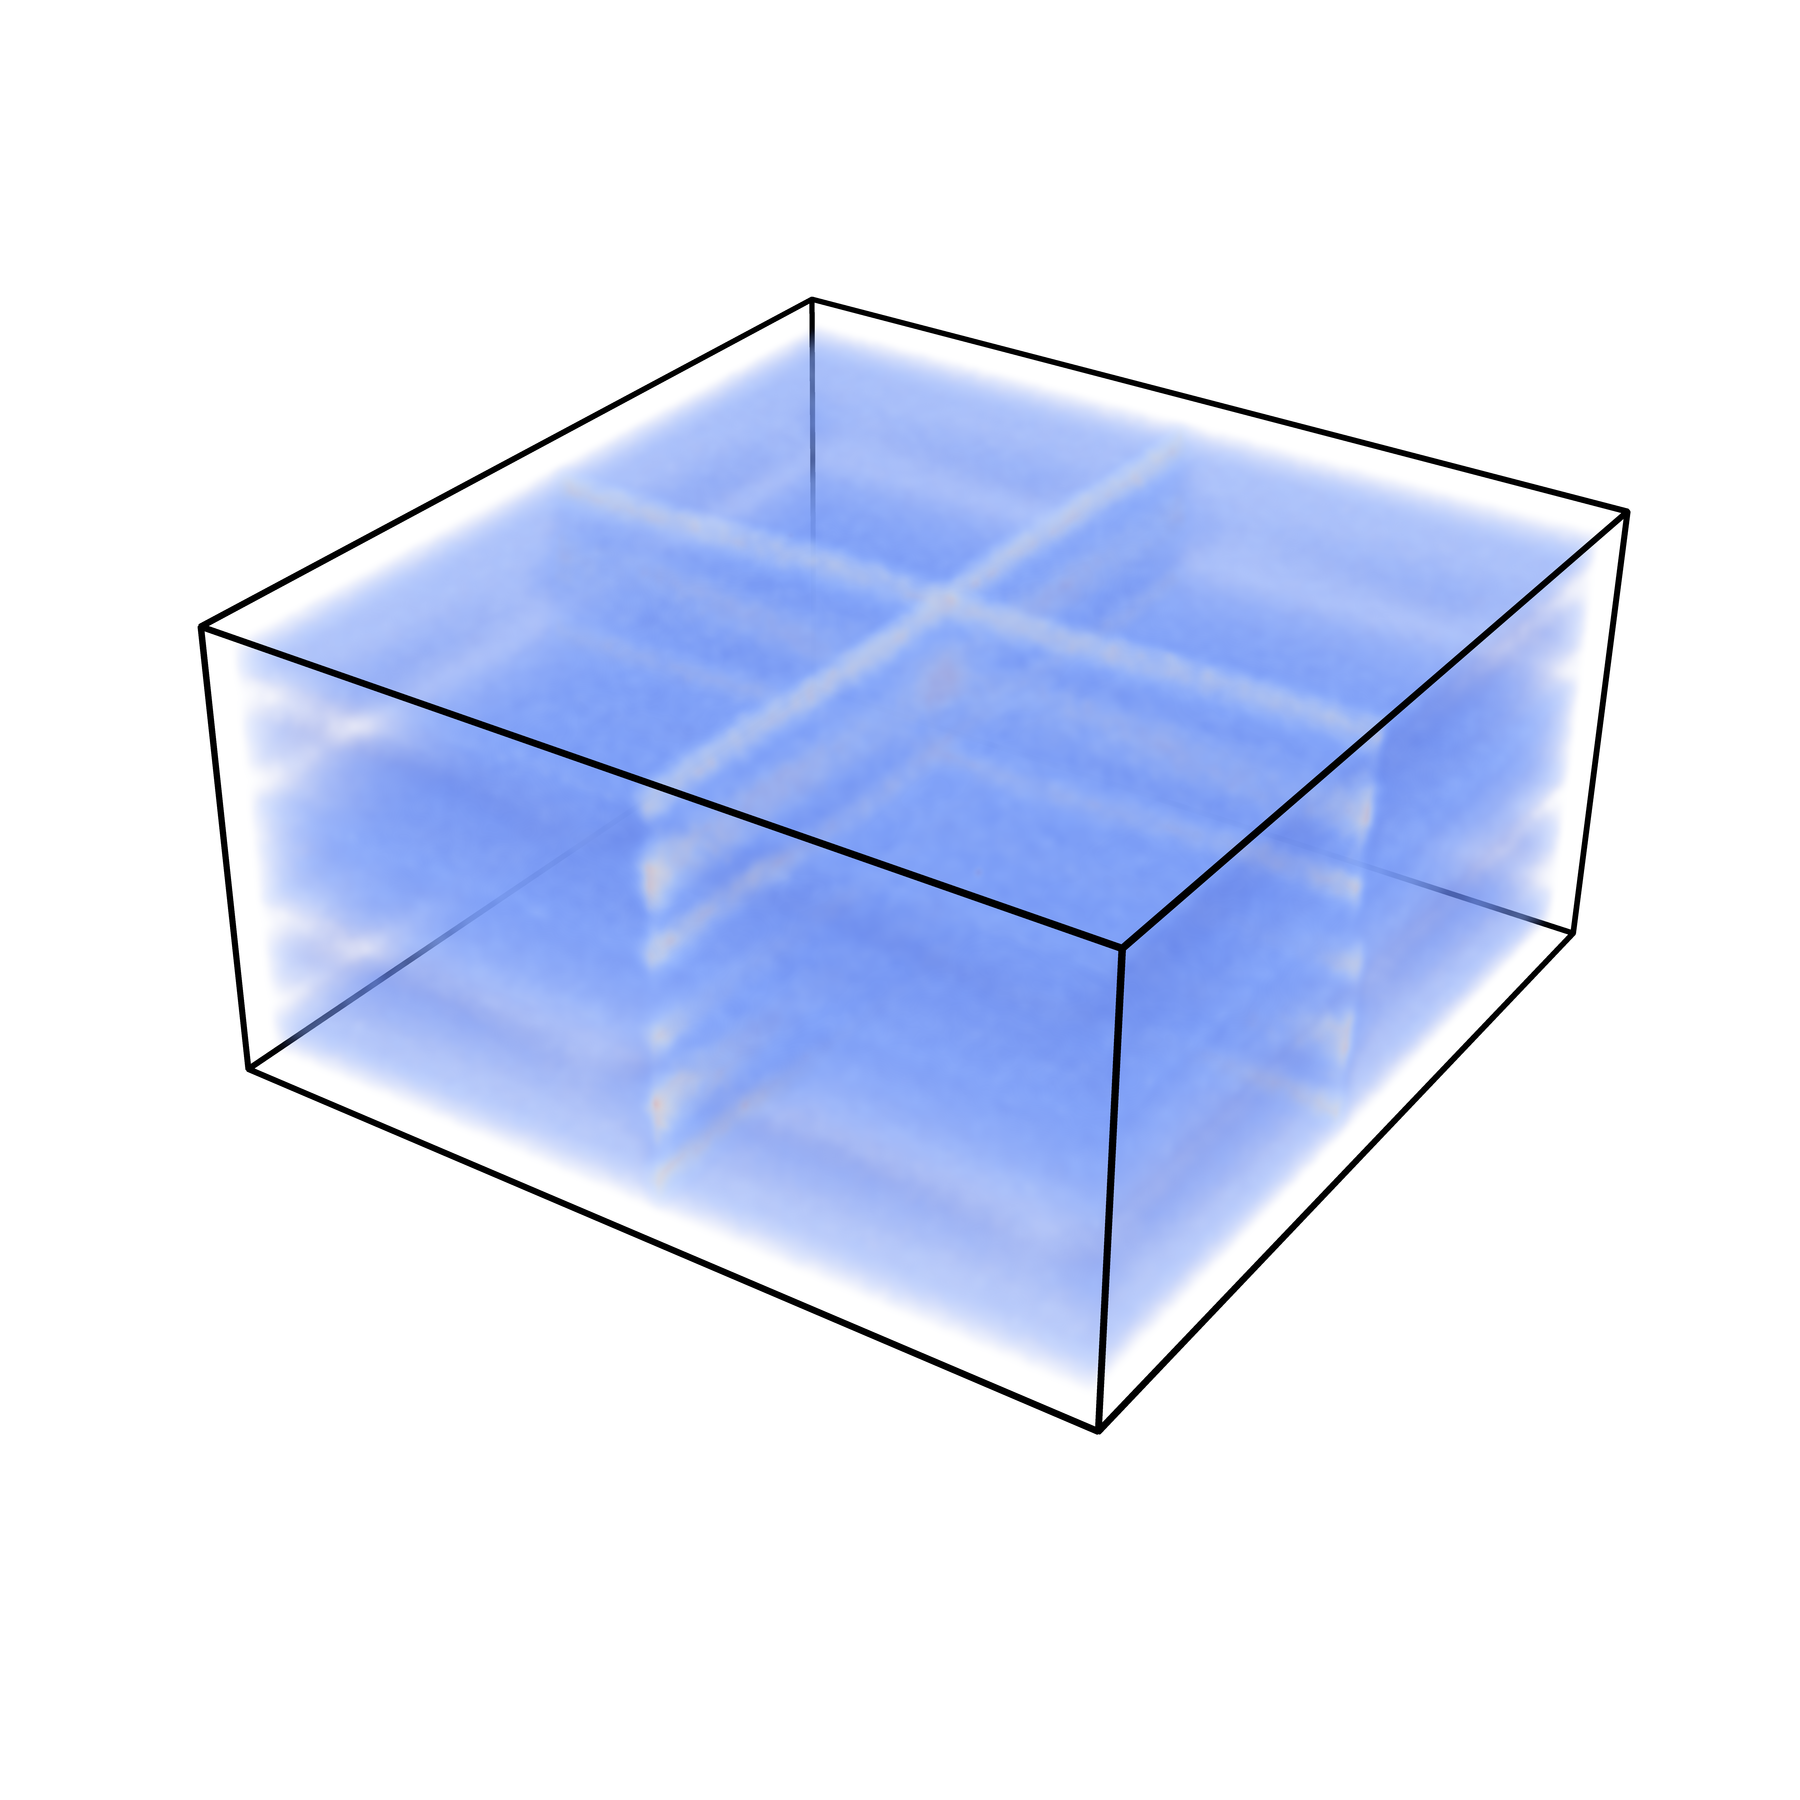
\includegraphics[width=\textwidth]{Images/highuncEigen.png}
        \caption{Eigendecomposition}
        \label{fig:HUCeigen}
    \end{subfigure}
    \begin{subfigure}[b]{0.49\textwidth}
        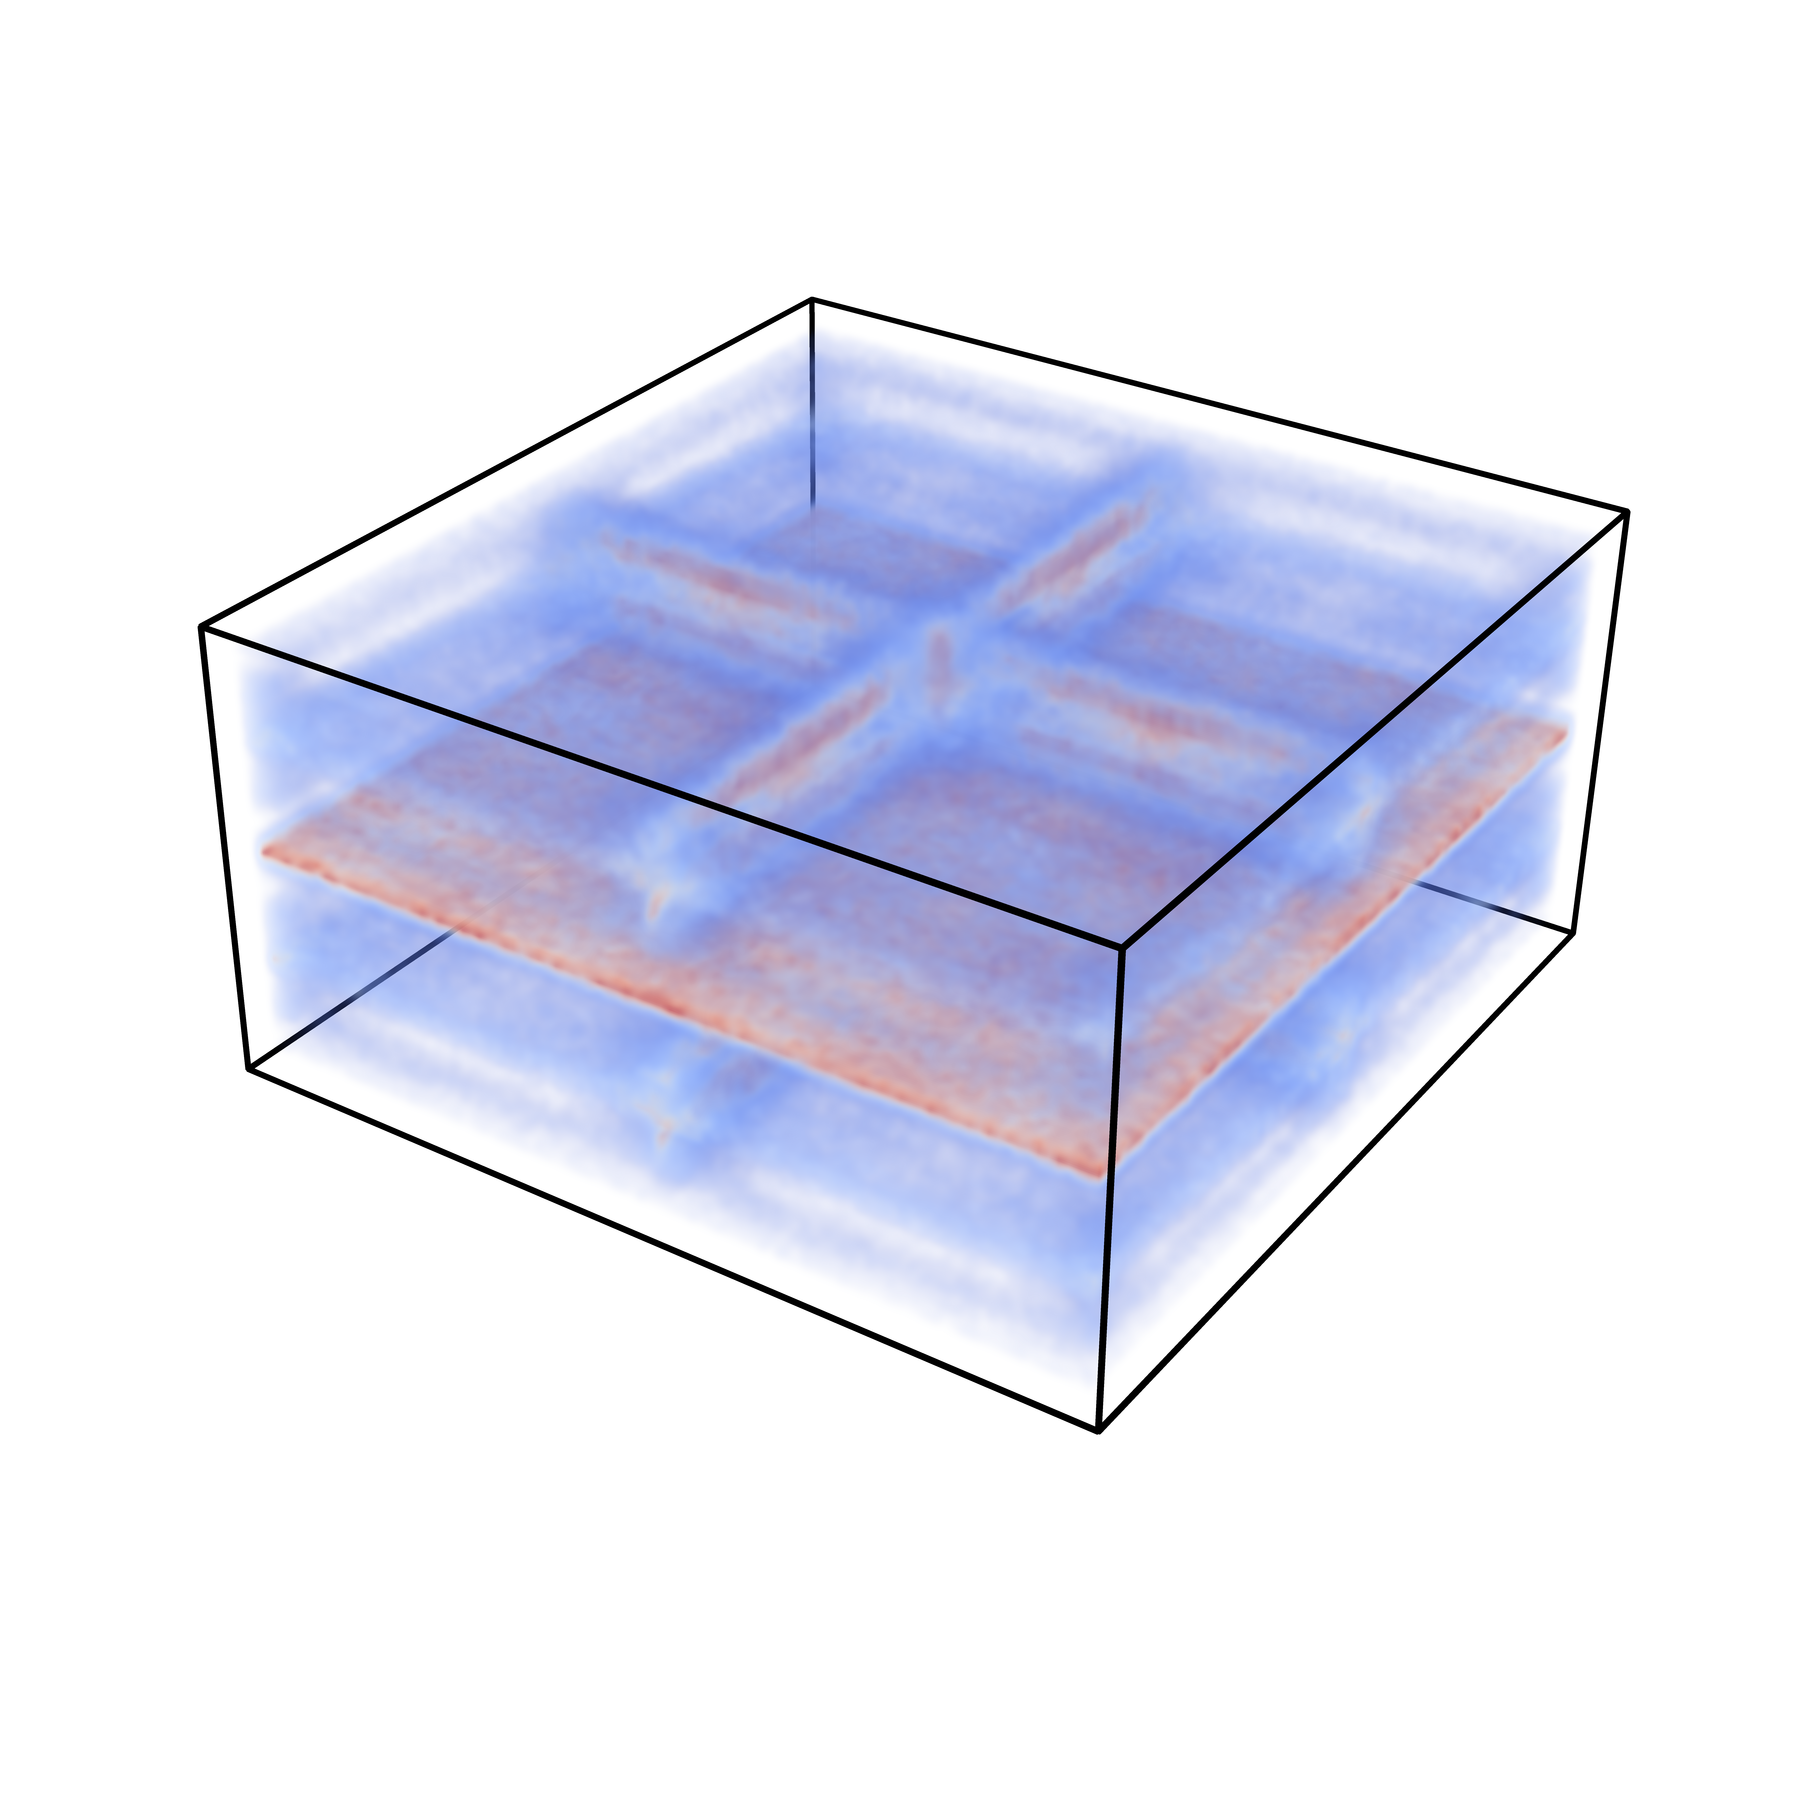
\includegraphics[width=\textwidth]{Images/highuncChol.png}
        \caption{Cholesky}
        \label{fig:HUCchol}
    \end{subfigure}
    \caption{Comparison of matrix decompositions for a set with high
    variance in every dimension. The Eigendecomposition exhibits a ridge
    structure appearing roughly around the mean, hardly distinguishable 
    from the noise surrounding it. Cholesky delivers a more certain
    structure, with holes in the cross like ridges on top and bottom,
    due to the up and downward distortion of the members.}
    \label{fig:HUCcomp}
\end{figure}
  %%%%%%%%%%%%%%%%%%%%%%%%%%%%%%%%%%%%%%%%%%%%%%%%%%%%%%%%%%%%%%%%%%%%%%%%
\chapter{Conclusion}\label{chap:Discu}
%%%%%%%%%%%%%%%%%%%%%%%%%%%%%%%%%%%%%%%%%%%%%%%%%%%%%%%%%%%%%%%%%%%%%%%%

This thesis took the idea of uncertain vortex core line detection and
transferred it to ridges in uncertain scalar fields. We deeply discussed
the adjustments to the considered neighborhood to achieve Gaussian
distributed derivatives and how the different approaches for the
generation of samples from the uncertain fields influence the results.\\
\indent While ridge lines in three dimensions almost directly follow the
work of Otto and Theisel, ridges of co-dimension one needed some
adjustments. As the conservative approach to extract the uncertain
ridges with a modification of the Marching Cubes algorithm yielded
problems at the locations where the ridge feature was weak already, we
made use of the information that eigenvectors give us about their
gradients, to develop a criterion that estimates the existence of a
ridge, rather than strictly calculating it. Essentially, the criterion
approximates the transformation of the gradient along the direction
perpendicular to a ridge with the directional derivatives denoted by the
eigenvalues, to estimate if the gradient in some distance $d$ flipped
its direction and therefore passed a ridge. This gave really smooth
results without undesired features, but with the downside of losing
precision, especially for mostly certain sets. There are a lot of
different ways to obtain the ridges, but the optimal parameters for the
extraction depend on the uncertainty of the data set, making general
recommendations difficult.\\
\indent For the future, a point wise implementation of the new criterion
should definitely be considered, as the criterion is independent of
neighboring nodes. This would only be more congruent with the overall
mechanism of the criterion. Furthermore this would challenge the
aliasing problem, occuring if the ridge is not aligned with an axis of
the grid, as well as reducing the arithmetical effort. For the
3-dimensional case, this would decrease the size of the covariance
matrix from $80 \times 80$ to $25 \times 25$ dimensional, boosting the
computation time and challenging the issues with the numerical stability
of either decomposition. Also, a filter should be implemented, that
changes the type of extracted feature, depending on their relevance at
the location. This is possible based on the eigenvalues, even together
with a point wise extraction and would further improove the results.\\
\indent The methods described in this work were implemented for discrete
scalar fields of identical resolution as a plugin for ParaView. With
this plugin, we produced our results we used to evaluate and compare
the different approaches.

}
% This ensures that the subsequent sections are being included as root
% items in the bookmark structure of your PDF reader.
\bookmarksetup{startatroot}
\backmatter{
  \printindex
  \printglossary{}
  \printbibliography{}
}
\end{document}
